\documentclass[a4paper,12pt]{article}

% ============================================================
%  IDIOMA E CODIFICAÇÃO
% ============================================================
\usepackage[utf8]{inputenc}
\usepackage[T1]{fontenc}
\usepackage[brazilian]{babel}
\frenchspacing

% ============================================================
%  MATEMÁTICA E QUÍMICA
% ============================================================
\usepackage{amsmath}
\usepackage{amssymb}
\usepackage[version=4]{mhchem}
\DeclareMathOperator{\sen}{sen}
\numberwithin{equation}{section}

% ============================================================
%  TABELAS
% ============================================================
\usepackage{array}
\usepackage{tabularx}
\usepackage{booktabs}
\usepackage{multirow}
\usepackage{longtable}
\usepackage[table]{xcolor}   % precisa vir antes do tikz/pgfplots
\usepackage{placeins}        % \FloatBarrier

% ============================================================
%  FIGURAS E GRÁFICOS
% ============================================================
\usepackage{graphicx}
\usepackage{float}           % permite [H]
\usepackage{tikz}
\usetikzlibrary{positioning, arrows.meta, fit, backgrounds,
                shapes.geometric, calc, patterns}
\usepackage{pgfplots}
\pgfplotsset{compat=1.18}
\usepackage{caption}
\captionsetup{skip=8pt}

% Cores usadas nos gráficos TikZ (Cap. 3)
\definecolor{corTransporte}{HTML}{2E75B6}
\definecolor{corBESS}{HTML}{1D9E75}
\definecolor{corOutros}{HTML}{A6A6A6}
\definecolor{corLinha}{HTML}{444444}

% Cores usadas no capítulo da fábrica
\definecolor{gigaAzul}{HTML}{2563EB}
\definecolor{gigaLaranja}{HTML}{D97706}
\definecolor{gigaVerde}{HTML}{16A34A}
\definecolor{gigaRoxo}{HTML}{7C3AED}
\definecolor{gigaCinza}{HTML}{6B7280}

% ============================================================
%  TEXTO, LAYOUT E DIVERSOS
% ============================================================
\usepackage{geometry}
\geometry{left=2cm, right=3cm, top=3cm, bottom=2cm, headheight=40pt}
\usepackage{enumitem}
\usepackage{wrapfig}
\usepackage{indentfirst}
\usepackage{changepage}
\usepackage{pdflscape}       % páginas em paisagem (Figura 9)
\usepackage{afterpage}       % insere a página em paisagem na próxima quebra
\usepackage{scalefnt}
\usepackage{soul}
\usepackage{ragged2e}
\usepackage{times}
\usepackage{siunitx}
\usepackage{gensymb}
\usepackage{courier}

% ============================================================
%  HYPERREF
% ============================================================
\usepackage{xurl}            % quebra de URLs longas nas referências
\usepackage[pdfusetitle,bookmarks=true,bookmarksopen=true,
            colorlinks=false,hidelinks]{hyperref}

% ============================================================
%  CITAÇÕES E REFERÊNCIAS (ABNT, sistema autor-data)
%  O abntex2cite deve ser carregado depois do hyperref.
% ============================================================
\usepackage[alf]{abntex2cite}

% ============================================================
%  CABEÇALHO E RODAPÉ
% ============================================================
\usepackage{fancyhdr}
\pagestyle{fancy}
\fancyhf{}
\fancyhead[L]{
\includegraphics[height=1cm]{Logo/logo_unicamp.png}}
\fancyhead[C]{\small Relatório Final de Iniciação Científica}
\fancyhead[R]{
\includegraphics[height=1cm]{Logo/Logo_FEM.png}}
\renewcommand{\headrulewidth}{0.4pt}
\fancyfoot[C]{\thepage}
\fancypagestyle{paisagem}{%
  \fancyhf{}%
  \renewcommand{\headrulewidth}{0pt}%
  \fancyfoot[C]{\thepage}}

% Nomenclatura em português
\addto\captionsbrazilian{\renewcommand{\tablename}{Tabela}}

% ============================================================
%  ESPAÇAMENTO
% ============================================================
\setlength{\parindent}{1.3cm}
\setlength{\parskip}{0.2cm}
\renewcommand{\arraystretch}{1.15}
\setlength{\tabcolsep}{6pt}
\setlength{\LTpre}{6pt}
\setlength{\LTpost}{12pt}
\setlength{\emergencystretch}{2em}  % reduz linhas que ultrapassam a margem

% ---------- Macro para fonte de tabelas/figuras ----------
\newcommand{\fonte}[1]{\par\vspace{3pt}{\footnotesize Fonte: #1}}

% ---------- Pendências de verificação (remover antes da entrega) ----------
% Marca, em vermelho no PDF, cada informação que depende de dado ou fonte
% ainda não confirmados. Para localizar todas: buscar "\pendente" no projeto.
\newcommand{\pendente}[1]{\textcolor{red}{[Pendente: #1]}}

% ---------- "Sem data" nas referências ABNT ----------
\DeclareRobustCommand{\sd}{[s.d.]}

% ============================================================
\begin{document}
\selectlanguage{brazilian}

% ----------------- PRÉ-TEXTUAIS -----------------
% Capa
\begin{titlepage}
\centering
  % logos lado a lado
  \makebox[\textwidth]{%
    
\includegraphics[height=0.9in]{Logo/logo_unicamp.png}%
    \hfill
    
\includegraphics[height=0.8in]{Logo/Logo_FEM.png}%
    }

\begin{center}
    {\scshape\LARGE Universidade Estadual de Campinas \par}
    {\scshape\Large Faculdade de Engenharia Mecânica \par}
    \vspace{2.2cm}
\end{center}

    {\large Relatório Final de Iniciação Científica\par}
    \vspace{0.9cm}
    {\LARGE\bfseries Fluxo de materiais da eletrificação da frota brasileira:
    químicas de bateria, cenários de frota e manufatura de células LFP\par}

    \vfill

    % Autores e orientador
    \begin{flushleft}
         \textbf{Autores}\\
         Enzo Godoy Canteri -- RA 278027\\
         Guilherme Diniz Santana -- RA 278092\\
         Lucas Lopes Baptistella -- RA 239022\\
         Níckolas Portela Dias da Silva -- RA 250914
    \end{flushleft}

    \begin{flushleft}
        \textbf{Orientador:} Prof. Joaquim Seabra
    \end{flushleft}

    \vspace{1.6cm}

    {\large Campinas \\ 2026\par}
\end{titlepage}

\begingroup
\renewcommand{\baselinestretch}{0.95} % Ajuste este número (0.9, 0.85, etc.) até caber
\setlength{\parskip}{0pt}             % Remove espaçamento entre parágrafos no sumário
\tableofcontents
\endgroup

\clearpage


% ----------------- TEXTUAIS -----------------
\newpage
\section{Introdução}
\label{sec:introducao}

\subsection{Contextualização}
\label{subsec:contextualizacao}

A transição para a mobilidade elétrica representa um dos maiores desafios de
escala industrial da atualidade, não apenas do ponto de vista energético, mas
sobretudo do ponto de vista de materiais. A demanda global por baterias de
íon-lítio ultrapassou a marca histórica de 1,0~TWh em 2024 e segue em trajetória
de crescimento acelerado, impulsionada tanto pela eletrificação do transporte
quanto pela expansão dos sistemas de armazenamento estacionário
(\textit{Battery Energy Storage Systems} -- BESS) \cite{McKinsey2026, IEA2025}.
Esse crescimento é acompanhado por uma diversificação intensa das químicas de
bateria -- NMC, LFP, LMFP, sódio-íon e estado sólido --, cada uma respondendo a
diferentes equilíbrios entre densidade energética, custo e segurança de
suprimento de materiais críticos.

Nesse cenário, a etapa de fim de vida das baterias ganha relevância crescente.
Estima-se que o volume global de baterias descartadas atinja aproximadamente
1,7~milhão de toneladas até 2030 \cite{melin2022} \pendente{conferir o valor na
fonte; em 2019, a mesma consultoria estimava 1,2~milhão de toneladas}, o que coloca a reciclagem e
o reaproveitamento de materiais críticos -- lítio, níquel, cobalto, manganês,
ferro e fósforo -- como uma peça central da sustentabilidade da própria
transição energética.

\subsection{Problema de Pesquisa}
\label{subsec:problema}

O Brasil ocupa uma posição particular nesse contexto global. Diferentemente da
Europa, cuja trajetória de eletrificação é liderada por veículos puramente
elétricos (BEV) de longo alcance, e da China, onde predominam BEV e híbridos
\textit{plug-in}, a frota brasileira sinaliza uma preferência consolidada por
rotas híbridas -- em especial o Híbrido-Flex (HEV) e o Híbrido \textit{Plug-in}
(PHEV) --, sustentada pela ampla disponibilidade de etanol e pela infraestrutura
de abastecimento já consolidada no país. Essa especificidade produz um perfil
químico próprio: na amostra de emplacamentos analisada neste trabalho
(Seção~\ref{sec:marketshare}), predomina o LFP, seguido do NMC, com uma parcela
expressiva de NiMH associada aos híbridos convencionais -- composição que difere
tanto da europeia, centrada no NMC, quanto da chinesa, centrada no LFP.

Embora a literatura internacional já disponha de estudos de Análise de Fluxo
de Materiais (MFA) para frotas eletrificadas europeias e chinesas, não se
identificaram estudos equivalentes que considerem a composição química
específica da frota brasileira nem os fluxos associados à fabricação de células
de bateria no país. Essa lacuna é agravada pela fragilidade do arcabouço
regulatório nacional: a legislação vigente -- a Política Nacional de Resíduos
Sólidos (Lei 12.305/2010) e a Resolução CONAMA 401/2008
\cite{pnrs2010,conama2008} -- não foi adaptada às especificidades das baterias
de tração de veículos elétricos, e o país ainda não dispõe de metas
quantitativas de reciclagem para essa categoria, ao contrário de China e União
Europeia.

\subsection{Objetivos}
\label{subsec:objetivos}

\subsubsection*{Objetivo Geral}

Caracterizar a frota eletrificada brasileira quanto às químicas de bateria e às
trajetórias de eletrificação até 2040 e quantificar, por meio de uma Análise de
Fluxo de Materiais e Energia (MEFA), os fluxos associados à fabricação de
células LFP -- a química mais frequente na frota --, como subsídio ao
planejamento da cadeia nacional de baterias e de reciclagem.

\subsubsection*{Objetivos Específicos}

\begin{enumerate}
    \item Estabelecer, a partir do cruzamento de dados de emplacamento da ABVE
    com as especificações técnicas do PBEV, a linha de base da participação
    (\textit{market share}) das químicas de bateria (LFP, NMC e NiMH) nos
    veículos eletrificados emplacados no país;

    \item Construir cenários de eletrificação da frota de veículos leves
    (Conservador e Acelerado) para os horizontes de 2030, 2035 e 2040, com base
    no estudo ANFAVEA/BCG e na verificação cruzada com as projeções do PDE 2035,
    da Bright Consulting e do MBC Brasil;

    \item Quantificar, por meio de uma MEFA de fronteira \textit{gate-to-gate},
    os fluxos de materiais, utilidades, emissões e resíduos da fabricação de
    células LFP, por kWh de célula e normalizados para 1~GWh de produção anual;

    \item Discutir as implicações dos resultados para a cadeia nacional de
    reciclagem, com ênfase na sucata de produção e nos gargalos econômicos e
    regulatórios identificados na literatura.
\end{enumerate}

A modelagem dinâmica dos estoques e fluxos de baterias da frota em uso, em fim
de vida e em segunda vida -- prevista no planejamento inicial do projeto -- não
integra o escopo deste relatório e é apresentada como continuidade do trabalho
no Capítulo~\ref{sec:conclusao}.

\subsection{Justificativa e Estrutura do Trabalho}
\label{subsec:justificativa}

A relevância deste trabalho decorre de três fatores complementares: (i) a
dependência brasileira de minerais críticos frequentemente importados, cuja
recuperação doméstica pode mitigar riscos de suprimento; (ii) o passivo
ambiental representado pelo descarte inadequado de baterias em fim de vida; e
(iii) a janela regulatória em aberto -- com projeto de lei em tramitação no
Senado Federal para instituir uma política nacional de circularidade das
baterias veiculares \cite{dialogueearth2026} --, que torna urgente a produção de
evidência técnica que subsidie a formulação dessa política.

O trabalho articula duas escalas de análise. Na escala da frota, caracteriza-se
o mercado brasileiro de veículos eletrificados quanto às químicas de bateria e
às trajetórias de eletrificação; na escala industrial, quantificam-se os fluxos
de materiais e energia de uma fábrica de células LFP, química mais frequente na
amostra analisada. As duas escalas se conectam pela química LFP e pela cadeia de
reciclagem, à qual a fábrica entrega um fluxo de material secundário homogêneo e
disponível desde o início da produção: a sucata de fabricação.

O relatório está estruturado da seguinte forma: o
Capítulo~\ref{sec:metodologia} descreve a metodologia das quatro frentes de
trabalho -- revisão bibliográfica, levantamento de \textit{market share},
construção dos cenários de frota e MEFA da fábrica; o
Capítulo~\ref{sec:revisao} revisa as tecnologias de bateria, a manufatura de
células e as rotas de reciclagem, segunda vida e regulação; o
Capítulo~\ref{sec:resultados} apresenta o \textit{market share}, os cenários de
frota e a transição para o estudo industrial; o Capítulo~\ref{sec:gigafabrica}
apresenta a MEFA da fábrica de células LFP; e o Capítulo~\ref{sec:conclusao}
sintetiza os resultados por objetivo, discute as limitações e aponta a
continuidade do trabalho.

\newpage
\section{Metodologia}
\label{sec:metodologia}

Este capítulo descreve as ferramentas e fontes utilizadas para produzir os
resultados apresentados ao longo do trabalho, organizadas em quatro frentes
metodológicas complementares: revisão bibliográfica estruturada, levantamento do
\textit{market share} das químicas de baterias, construção dos cenários de frota
e Análise de Fluxo de Materiais e Energia (MEFA) de uma fábrica de células LFP.
As três primeiras frentes operam na escala da frota; a quarta, na escala
industrial.

% ===========================================================
\subsection{Revisão Bibliográfica}
\label{sec:met-revisao}
% ===========================================================

A revisão bibliográfica foi conduzida de forma estruturada nas bases de dados
\textbf{Scopus}, \textbf{Web of Science} e \textbf{ScienceDirect}, com cobertura
temporal principal entre 2021 e 2025, de modo a capturar os avanços mais recentes
em um setor de rápida evolução tecnológica. Por não seguir um protocolo
sistemático de seleção (com critérios formais de inclusão e exclusão e
contagem dos documentos triados), a revisão é caracterizada como estruturada.

As buscas foram organizadas em três eixos temáticos:

\begin{enumerate}
    \item \textbf{Química e tecnologia de baterias:} as palavras-chave utilizadas
    incluíram termos como \textit{lithium-ion battery}, \textit{LFP}, \textit{NMC},
    \textit{sodium-ion battery}, \textit{solid-state battery} e \textit{battery
    technology roadmap}. Foram priorizados artigos de revisão com alto número de
    citações, relatórios técnicos de organismos internacionais — como a Agência
    Internacional de Energia (IEA) e o consórcio europeu EUROBAT — e estudos de
    modelagem tecno-econômica que aplicam curvas de aprendizado
    (\textit{Lei de Wright}) para projeção de custos de pacotes de baterias.

    \item \textbf{Processos de reciclagem de baterias de íon-lítio:} as
    palavras-chave empregadas foram \textit{lithium-ion battery recycling},
    \textit{hydrometallurgy spent batteries}, \textit{pyrometallurgy LIB},
    \textit{direct recycling cathode}, \textit{LFP recycling economic},
    \textit{second-life battery} e \textit{battery recycling regulation Brazil}.
    Foram priorizados artigos de revisão abrangentes, estudos de avaliação de ciclo
    de vida e análises tecno-econômicas comparativas, bem como relatórios técnicos
    do Laboratório Nacional de Energia Renovável dos EUA (NREL) e fontes
    regulatórias nacionais.

    \item \textbf{Manufatura de células:} relatórios técnicos e estudos de custo e
    de fluxo de energia da produção de células de íon-lítio
    \cite{knehr2022batpac,degen2022,erakca2021,dai2019}, que fundamentam a MEFA
    descrita na Seção~\ref{sec:met-mefa}.
\end{enumerate}

Para a avaliação da maturidade tecnológica das diferentes químicas e rotas de
reciclagem, adotou-se a escala de \textit{Technology Readiness Level} (TRL),
seguindo a classificação do roteiro EUROBAT para baterias automotivas
(Gerações~3, 4 e~5).

% ===========================================================
\subsection{Levantamento do \textit{Market Share} de Químicas}
\label{sec:met-marketshare}
% ===========================================================

A determinação da participação de mercado das diferentes químicas de baterias na
frota eletrificada brasileira baseou-se no cruzamento de duas fontes de dados
primários:

\begin{itemize}
    \item \textbf{Dados de emplacamentos da ABVE:} registros de vendas de veículos
    eletrificados (BEV, PHEV e HEV) fornecidos pela Associação Brasileira do
    Veículo Elétrico \cite{ABVE}, que constituíram a base quantitativa do estudo.

    \item \textbf{Especificações técnicas do PBEV:} fichas técnicas do Programa
    Brasileiro de Etiquetagem Veicular \cite{PBEV}, utilizadas para identificar
    a química de bateria de cada modelo comercializado no mercado nacional.
\end{itemize}

A metodologia consistiu em (i)~selecionar os modelos de maior impacto em volume de
vendas, segmentados por categoria (BEV, PHEV e HEV); (ii)~atribuir a cada modelo a
respectiva química de bateria com base nas fichas do PBEV e, quando necessário, em
informações técnicas dos fabricantes; e (iii)~consolidar os dados em uma amostra
de \textbf{mais de 509\,mil veículos eletrificados}, a partir da qual foram
calculadas as proporções de cada tecnologia — LFP, NMC e NiMH. O período de
emplacamentos coberto pela base é
\pendente{informar o período da base ABVE (BI Geral) e a data da consulta}.

As participações são calculadas em número de veículos emplacados e, portanto,
não equivalem à participação em massa de baterias ou em capacidade (kWh): o
pacote de um híbrido convencional tem da ordem de 1 a 2~kWh, e o de um BEV,
dezenas de kWh (Seção~\ref{subsec:contexto-brasil}). Essa linha de base
caracteriza a composição química das baterias que circularão e serão
descartadas no país e orienta a escolha da química LFP para o estudo industrial
(Seção~\ref{sec:met-mefa}).

% ===========================================================
\subsection{Construção dos Cenários de Frota}
\label{sec:met-cenarios}
% ===========================================================

Para estabelecer as projeções de eletrificação da frota automotiva brasileira com
horizontes em 2030, 2035 e 2040, foram analisados quatro documentos institucionais
de referência:

\begin{enumerate}
    \item \textbf{ANFAVEA/BCG:} estudo da Associação Nacional dos Fabricantes de
    Veículos Automotores com o \textit{Boston Consulting Group}, divulgado em
    2024, que apresenta dois cenários de eletrificação — transição gradual e
    transição acelerada — para os horizontes de 2030, 2035 e 2040
    \cite{anfaveabcg2024}.

    \item \textbf{PDE 2035 — Plano Decenal de Expansão de Energia}
    \cite{EPE2025}: projeções governamentais de vendas e frota circulante de
    veículos leves e pesados, com detalhamento do eixo de eletromobilidade.

    \item \textbf{Bright Consulting:} previsões de mercado e frota com horizonte
    principal em 2030, com foco na trajetória de hibridização da frota brasileira
    \cite{BrightConsulting}.

    \item \textbf{MBC Brasil — Movimento Brasil Competitivo:} estudo sobre
    transição energética da mobilidade de baixo carbono no Brasil com horizonte em
    2040 \cite{MBCBrasil}.
\end{enumerate}

Diante da disparidade numérica entre as projeções, adotou-se como espinha
dorsal o estudo ANFAVEA/BCG — única fonte consultada que apresenta dois cenários
e os três horizontes de interesse — e as demais fontes foram usadas como
verificação cruzada de ordem de grandeza:

\begin{itemize}
    \item \textbf{Cenário Conservador:} corresponde ao cenário de transição gradual
    do estudo ANFAVEA/BCG, com predominância do Híbrido-Flex e gargalos de
    infraestrutura de recarga.

    \item \textbf{Cenário Acelerado:} corresponde ao cenário de transição
    acelerada, com maior penetração de BEV e PHEV, associada à efetividade de
    programas como o \textit{Mover} e o \textit{Novo PAC}.
\end{itemize}

Os valores por categoria e horizonte são reproduzidos da fonte, arredondados ao
milhão (Seção~\ref{subsec:cenarios-sensibilidade}). As projeções do PDE 2035, da
Bright Consulting e do MBC Brasil são comparadas a eles no mesmo horizonte,
distinguindo-se, quando possível, a inclusão ou não dos híbridos leves (MHEV).

Os veículos pesados não integram a quantificação dos cenários. Para os
caminhões, as projeções consultadas indicam predominância do diesel ao longo do
horizonte (Seção~\ref{subsec:pesados}); para os ônibus, embora a eletrificação
urbana seja relevante, as fontes consultadas não oferecem séries comparáveis às
dos veículos leves para os três horizontes. Os cenários quantitativos
concentram-se, portanto, nos \textbf{veículos leves}.

% ===========================================================
\subsection{Análise de Fluxo de Materiais e Energia da Fábrica}
\label{sec:met-mefa}
% ===========================================================

A Análise de Fluxo de Materiais (MFA) é um sistema de equações de balanço de
massa aplicado a processos e fluxos delimitados no espaço e no tempo
\cite{BrunnerRechberger}. Neste trabalho, o método é aplicado a uma fábrica de
células LFP e estendido aos fluxos de energia e de utilidades — eletricidade,
água e gases técnicos —, à semelhança da análise de fluxos de energia aplicada
por \citeonline{erakca2021} à produção de células; por isso, adota-se a
denominação Análise de Fluxo de Materiais e Energia (MEFA). Os elementos do
método são:

\begin{itemize}
    \item \textbf{Unidade funcional:} 1~kWh de célula LFP acabada e testada, em
    formato prismático, com densidade energética de referência de 160~Wh/kg
    (6,25~kg de célula por kWh).

    \item \textbf{Base de normalização:} os resultados por kWh são multiplicados
    por $10^{6}$ e expressos por GWh de células produzidas por ano. A
    normalização não representa a capacidade física de uma planta específica: os
    parâmetros correspondem a uma planta madura em operação consolidada, e plantas
    pequenas ou em \textit{ramp-up} apresentam intensidades energéticas superiores
    (Seção~\ref{subsec:giga-indicadores}).

    \item \textbf{Fronteira:} do tipo \textit{gate-to-gate}, do recebimento das
    matérias-primas no portão da fábrica até a expedição das células acabadas; as
    inclusões e exclusões são detalhadas na Seção~\ref{subsec:giga-bases}.

    \item \textbf{Fontes:} faixas de referência da literatura técnica de
    manufatura de células \cite{knehr2022batpac,degen2022,erakca2021,dai2019};
    não há medições de uma planta específica.

    \item \textbf{Tratamento das faixas:} cada parâmetro é registrado com a faixa
    da literatura e um valor central adotado para o balanço. Os valores são
    classificados como \textbf{L} (dado de literatura), \textbf{H} (hipótese
    adotada neste trabalho) ou \textbf{C} (calculado a partir de L e H),
    classificação indicada nas tabelas do Capítulo~\ref{sec:gigafabrica}.

    \item \textbf{Balanços:} em regime permanente, para cada processo $i$,
    \begin{equation}
        \sum_{j} \dot{m}^{\,\text{entrada}}_{i,j} = \sum_{k} \dot{m}^{\,\text{saída}}_{i,k},
        \label{eq:balanco}
    \end{equation}
    e o balanço global resulta da composição dos balanços por etapa, aplicados aos
    materiais que efetivamente atravessam cada etapa.

    \item \textbf{Classificação dos fluxos:} (a) entradas externas, que cruzam a
    fronteira vindas de fornecedores; (b) saídas externas — produto, subprodutos,
    resíduos, emissões e efluentes; e (c) circuitos internos, que deixam uma
    etapa e retornam ao processo sem cruzar a fronteira (recuperação de NMP,
    retorno de pasta, recirculação de água e de energia).
\end{itemize}

% ===========================================================
\subsection{Síntese da Abordagem Metodológica}
\label{sec:met-sintese}
% ===========================================================

A Figura~\ref{fig:fluxo-metodologico} ilustra a integração entre as quatro
frentes. Na escala da frota, os dados de emplacamento (ABVE/PBEV) alimentam o
\textit{market share}, e os documentos institucionais alimentam os cenários. Na
escala industrial, a literatura de manufatura alimenta a MEFA da fábrica, cuja
química decorre do \textit{market share}. As duas escalas convergem, com o
contexto tecnológico e regulatório da revisão bibliográfica, para a discussão das
implicações para a cadeia de reciclagem. A modelagem dinâmica dos fluxos da frota (MFA em uso, fim de vida
e segunda vida) é indicada como etapa futura.

\begin{figure}[H]
\centering
\resizebox{\textwidth}{!}{%
\begin{tikzpicture}[
    box/.style   = {rectangle, rounded corners, draw=black!60, thick,
                    fill=gray!8, align=flush center, minimum height=1.1cm,
                    text width=3.3cm, font=\footnotesize},
    fonte/.style = {box, fill=blue!6},
    res/.style   = {box, fill=orange!10},
    ind/.style   = {box, fill=green!10},
    sint/.style  = {box, fill=purple!8, text width=3.0cm, minimum height=2.6cm},
    fut/.style   = {box, dashed, fill=white, draw=black!50, text=black!70,
                    text width=3.0cm},
    arrow/.style = {-{Latex[length=2.6mm]}, thick},
    darrow/.style= {-{Latex[length=2.6mm]}, thick, dashed, black!55},
]
% --- escala da frota
\node[fonte] (inst) at (0, 0)    {Documentos institucionais\\(ANFAVEA/BCG, PDE, Bright, MBC)};
\node[fonte] (abve) at (0,-1.9)  {ABVE / PBEV\\(emplacamentos\\e fichas)};
\node[res]   (cen)  at (5, 0)    {Cenários de frota\\(2030, 2035, 2040)};
\node[res]   (ms)   at (5,-1.9)  {\textit{Market share}\\das químicas};
% --- escala industrial
\node[fonte] (man)  at (0,-4.2)  {Literatura de manufatura\\de células};
\node[ind]   (mefa) at (5,-4.2)  {MEFA da fábrica\\de células LFP};
% --- revisão
\node[fonte] (lit)  at (0,-6.1)  {Literatura científica\\e técnica};
\node[box]   (rev)  at (5,-6.1)  {Revisão\\bibliográfica};
% --- molduras de escala
\begin{scope}[on background layer]
\node[draw=black!30, dashed, rounded corners, inner sep=7pt, fill=gray!3,
      fit=(inst)(abve)(cen)(ms),
      label={[font=\scriptsize\bfseries, anchor=south west]north west:Escala da frota}]
      (frota) {};
\node[draw=black!30, dashed, rounded corners, inner sep=7pt, fill=gray!3,
      fit=(man)(mefa),
      label={[font=\scriptsize\bfseries, anchor=south west]north west:Escala industrial}]
      (industria) {};
\end{scope}
% --- síntese e etapa futura
\node[sint] (impl) at (10.3,-3.05) {Implicações\\para a cadeia\\de reciclagem};
\node[fut]  (mfa)  at (10.3, 0.35) {MFA dinâmico\\da frota\\(etapa futura)};
% --- setas
\draw[arrow] (inst) -- (cen);
\draw[arrow] (abve) -- (ms);
\draw[arrow] (man)  -- (mefa);
\draw[arrow] (lit)  -- (rev);
\draw[arrow] (ms) -- node[right=2pt, font=\scriptsize, align=left] {química LFP} (mefa);
\draw[arrow] (frota.east |- 0,-2.0) -- (impl.west |- 0,-2.0);
\draw[arrow] (industria.east |- mefa.east) -- (impl.west |- mefa.east);
\draw[arrow] (rev.east) -| (impl.south);
\draw[darrow] (frota.east |- mfa.west) -- (mfa.west);
\end{tikzpicture}%
}
\caption{Fluxo metodológico integrado da pesquisa. Setas tracejadas indicam a
         etapa futura (MFA dinâmico da frota), fora do escopo deste relatório.}
\label{fig:fluxo-metodologico}
\end{figure}

\newpage
\section{Revisão Bibliográfica e Contexto Tecnológico}
\label{sec:revisao}

Esta revisão organiza-se em três blocos. O primeiro (Seções~\ref{sec:contexto}
e~\ref{sec:quimicas}) examina o contexto de mercado e as químicas de bateria
relevantes para a frota brasileira. O segundo (Seção~\ref{sec:manufatura})
descreve a cadeia de fabricação de células, base do estudo industrial do
Capítulo~\ref{sec:gigafabrica}. O terceiro (Seção~\ref{sec:reciclagem}) revisa
as rotas de reciclagem, a segunda vida e o panorama regulatório, que fundamentam
a discussão das implicações para a cadeia nacional de reciclagem.

% ===========================================================
\subsection{Contexto Energético Global e Nacional}
\label{sec:contexto}
% ===========================================================

\subsubsection{Demanda, Supercapacidade e Custos}
\label{subsec:escala-global}

Segundo a McKinsey \cite{McKinsey2026}, a demanda global por baterias de
íon-lítio, que ultrapassou \textbf{1{,}0~TWh} em 2024, deveria atingir
\textbf{1{,}6~TWh} em 2025. O crescimento apoia-se em dois pilares: a
eletrificação do transporte, maior consumidor de baterias, e o armazenamento
estacionário (BESS), segmento de maior crescimento relativo, essencial para
integrar fontes renováveis intermitentes à rede. A
Figura~\ref{fig:demanda-global-baterias} ilustra a evolução histórica e
projetada por segmento. A série de transporte da figura indica cerca de
2{,}2~TWh em 2030, abaixo do patamar superior a 3{,}0~TWh anuais citado para o
cenário \textit{Stated Policies} da Agência Internacional de Energia
\cite{IEA2025}, diferença que reflete as fontes e os cenários adotados
\pendente{identificar a fonte de cada série da Figura~\ref{fig:demanda-global-baterias}}.

\begin{figure}[H]
\centering
\begin{tikzpicture}
\begin{axis}[
    width  = 15.5cm,
    height = 7.8cm,
    ybar stacked,
    bar width = 11pt,
    xtick          = {0,1,2,3,4,5,6,7,8,9,10,11,12,13,14,15},
    xticklabels    = {2020,2021,2022,2023,2024,2025,2026,2027,2028,
                      2029,2030,2031,2032,2033,2034,2035},
    x tick label style = {rotate=45, anchor=east, font=\footnotesize},
    xmin = -0.7, xmax = 15.7,
    ymin = 0, ymax = 6.3,
    ylabel         = {Demanda global (TWh)},
    ylabel style   = {font=\footnotesize},
    ytick          = {0,1,2,3,4,5,6},
    yticklabel     = {\pgfmathprintnumber[fixed,precision=1]{\tick}},
    yticklabel style = {font=\footnotesize},
    ymajorgrids    = true,
    grid style     = {dotted, gray!35},
    axis line style = {gray!60, line width=0.5pt},
    axis x line*    = bottom,
    axis y line*    = left,
    legend style = {
        at                = {(0.5,-0.34)},
        anchor            = north,
        font              = \footnotesize,
        draw              = none,
        fill              = none,
        legend columns    = 3,
        column sep        = 12pt,
        legend cell align = left,
    },
    clip = false,
]

\addplot[fill=corTransporte, draw=none] coordinates {
    (0,0.145) (1,0.240) (2,0.395) (3,0.585) (4,0.720) (5,1.100)
    (6,1.380) (7,1.620) (8,1.860) (9,2.050) (10,2.200) (11,2.430)
    (12,2.650) (13,2.860) (14,3.060) (15,3.250)
};
\addlegendentry{Transporte (veículos)}

\addplot[fill=corBESS, draw=none, postaction={pattern=north east lines, pattern color=white!70!corBESS}] coordinates {
    (0,0.018) (1,0.040) (2,0.080) (3,0.135) (4,0.190) (5,0.350)
    (6,0.500) (7,0.650) (8,0.780) (9,0.920) (10,1.060) (11,1.210)
    (12,1.370) (13,1.540) (14,1.710) (15,1.890)
};
\addlegendentry{Armazenamento estacionário (BESS)}

\addplot[fill=corOutros, draw=none] coordinates {
    (0,0.027) (1,0.040) (2,0.055) (3,0.070) (4,0.090) (5,0.150)
    (6,0.190) (7,0.230) (8,0.270) (9,0.320) (10,0.370) (11,0.420)
    (12,0.470) (13,0.520) (14,0.570) (15,0.610)
};
\addlegendentry{Outros (eletrônicos, indústria)}

% Rótulos de total em anos-chave
\node[font=\tiny, text=black!75, anchor=south] at (axis cs: 0,  0.34) {0,19};
\node[font=\tiny, text=black!75, anchor=south] at (axis cs: 5,  1.75) {1,60};
\node[font=\tiny, text=black!75, anchor=south] at (axis cs: 10, 3.78) {3,63};
\node[font=\tiny, text=black!75, anchor=south] at (axis cs: 15, 5.90) {5,75};

% Linha de início das projeções (2026)
\draw[corLinha, dashed, line width=0.9pt, dash pattern=on 4pt off 3pt]
    (axis cs: 5.5, 0) -- (axis cs: 5.5, 6.0);
\draw[-{Latex[length=4pt]}, corLinha, line width=0.7pt]
    (axis cs: 5.6, 5.85) -- (axis cs: 7.0, 5.85);
\node[anchor=west, font=\footnotesize\bfseries, text=corLinha]
    at (axis cs: 5.65, 6.10) {Projetado};

\end{axis}
\end{tikzpicture}

\caption{Demanda global por baterias de íon-lítio por segmento de aplicação
         (2020--2035). Valores a partir de 2026 são projetados.}
\label{fig:demanda-global-baterias}
\fonte{adaptado de \citeonline{McKinsey2026} e \citeonline{IEA2025}.}
\end{figure}

Simultaneamente, o mercado atravessa um período de \textbf{supercapacidade
produtiva}, concentrada na Ásia: em 2025, a oferta instalada excedeu a demanda em
aproximadamente 900~GWh, e o custo médio dos pacotes atingiu a mínima histórica de
\textbf{US\$~108/kWh}, redução superior a 50\% em relação a 2018
\cite{McKinsey2026}. Projeções baseadas na \textit{Lei de Wright} — que relaciona
a redução de custos ao volume acumulado de produção — indicam que os pacotes
LFP/LMFP podem chegar a \textbf{US\$~55 a 65/kWh até 2035}, assumindo preços
estáveis de matérias-primas e ganhos de eficiência em processos como o
revestimento de eletrodos a seco (\textit{dry coating}) \cite{EUROBAT}.

A queda de preços tem duplo efeito. De um lado, acelera a paridade de custo total
de propriedade (\textit{Total Cost of Ownership} — TCO) entre veículos elétricos
e a combustão, inclusive em mercados emergentes como o Brasil; de outro, reduz o
valor relativo dos materiais recuperados pela reciclagem, sobretudo nas químicas
de menor valor intrínseco, como a LFP (Seção~\ref{subsec:lfp-economics}). A
pressão sobre as cadeias de lítio, níquel e cobalto — minerais de distribuição
geográfica concentrada e mercados instáveis — impulsiona ainda a diversificação
das químicas: a migração do NMC para o LFP em segmentos de volume, o surgimento
do LMFP, o desenvolvimento do sódio-íon e a entrada gradual das baterias em
estado sólido (Seção~\ref{sec:quimicas}).

\subsubsection{O Contexto Energético Brasileiro}
\label{subsec:contexto-brasil}

O Brasil ocupa uma posição particular na transição para a mobilidade elétrica,
condicionada por três fatores estruturais que moldam o perfil de sua frota
eletrificada e, consequentemente, o fluxo de materiais de baterias.

\paragraph{A rota híbrida flex como caminho próprio.}
Enquanto a Europa e a China priorizam veículos puramente elétricos (BEV) e
híbridos \textit{plug-in}, a frota nacional sinaliza uma preferência por
veículos urbanos de baixo custo e por rotas híbridas — em particular os
Híbridos-Flex (HEV Flex) e os Híbridos \textit{Plug-in} (PHEV). Essa preferência
decorre da ampla disponibilidade de etanol e da vasta infraestrutura de postos de
combustível. Nesse contexto, os Veículos Elétricos com Extensor de Autonomia
(REEV — \textit{Range Extended Electric Vehicle}) surgem como alternativa
promissora, pois operam primariamente em modo elétrico e utilizam o etanol como
fonte secundária de energia \cite{BrightConsulting}.

\paragraph{A predominância de modelos asiáticos de entrada.}
A expansão da mobilidade elétrica no Brasil é tracionada majoritariamente por
montadoras asiáticas — especialmente BYD, GWM e JAC —, que priorizam as químicas
LFP e NMC para reduzir o preço final ao consumidor em um mercado sensível a
custo. A composição química resultante na amostra analisada neste trabalho é
apresentada na Seção~\ref{sec:marketshare}.

\paragraph{A implicação direta para o fluxo de materiais.}
As baterias de híbridos convencionais são significativamente menores do que as
de veículos puramente elétricos: um HEV típico opera com um pacote de 1 a 2~kWh,
enquanto um BEV popular carrega entre 30 e 80~kWh. A demanda por lítio e demais
minerais críticos por veículo é, portanto, menor no cenário brasileiro do que
seria em uma eletrificação plena baseada em BEV. Essa vantagem por unidade não
elimina a necessidade de uma infraestrutura de reciclagem e logística reversa,
uma vez que o volume acumulado de baterias em fim de vida crescerá de forma
contínua ao longo das próximas décadas \cite{EPE2025,MBCBrasil}. A
Tabela~\ref{tab:comparativo-mercados} sintetiza as diferenças entre a trajetória
brasileira e as dos principais mercados de referência.

\begin{table}[H]
    \centering
    \caption{Comparativo da trajetória de eletrificação: Brasil vs.\ mercados
             globais de referência.}
    \label{tab:comparativo-mercados}
    \renewcommand{\arraystretch}{1.4}
    \small
    \rowcolors{2}{gray!10}{white}
    \begin{tabularx}{\textwidth}{
        >{\raggedright\arraybackslash}p{3.6cm}
        >{\raggedright\arraybackslash}X
        >{\raggedright\arraybackslash}X
        >{\raggedright\arraybackslash}X }
    \toprule
    \textbf{Dimensão} & \textbf{Brasil} & \textbf{Europa} & \textbf{China} \\
    \midrule
    Tecnologia dominante & Híbrido-Flex (HEV) e PHEV & BEV de longo alcance & BEV e PHEV \\
    Química predominante & LFP, seguido de NMC e NiMH (Seção~\ref{sec:marketshare}) & NMC (45\%+) & LFP ($>$55\%) \\
    Combustível alternativo & Etanol (flex) & -- & -- \\
    Horizonte de 30\% da frota eletrificada & $\sim$2040 & $\sim$2030 & Já superado em regiões-chave \\
    Principal indutor & Programas Mover e Novo PAC & Regulação de CO$_2$ e fim dos ICE & Subsídios diretos e mandatos \\
    \bottomrule
    \end{tabularx}
    \fonte{elaborada pelos autores \pendente{indicar as fontes dos valores de Europa e China}.}
\end{table}

% ===========================================================
\subsection{Química das Baterias}
\label{sec:quimicas}
% ===========================================================

A escolha da química de bateria determina a densidade energética disponível por
veículo, o custo por kWh, os riscos da cadeia de suprimentos e, sobretudo, a
composição dos materiais que futuramente entrarão no fluxo de reciclagem. Esta
seção revisa as químicas presentes na frota brasileira — NMC, LFP/LMFP e NiMH —
e, de forma resumida, as tecnologias emergentes de sódio-íon e estado sólido.

\subsubsection{NMC (Níquel-Manganês-Cobalto)}
\label{subsec:nmc}

As baterias NMC consolidaram-se como o padrão de alto desempenho para veículos de
longo alcance e segmentos \textit{premium}, pela elevada densidade energética. A
família é caracterizada pela proporção de níquel, manganês e cobalto no cátodo; ao
longo da última década, a indústria migrou da composição original NMC~111 (um
terço de cada metal) para as variantes NMC~532 e NMC~622 e, depois, para o
NMC~811 (80\% Ni, 10\% Mn e 10\% Co), de maior densidade energética e maior
sensibilidade térmica, com o NMC de alto manganês como direção futura.

A dependência de cobalto e níquel expõe o NMC à volatilidade de preços e a riscos
geopolíticos: a República Democrática do Congo responde por mais de 70\% da
produção mundial de cobalto \cite{IEA2025}, e o níquel de alta pureza é
majoritariamente produzido na Indonésia e nas Filipinas. Projeta-se que o NMC
represente entre 43\% e 45\% da demanda na União Europeia e na América do Norte
até 2035 \cite{McKinsey2026}. No Brasil, sensível a preço, a química tende a
ocupar um nicho — veículos de alta performance, PHEVs de categorias superiores e
frotas de longo curso —, embora seja a segunda mais frequente na amostra
analisada, com presença expressiva em modelos da GWM, Volvo e CAOA Chery
(Seção~\ref{sec:marketshare}).

\subsubsection{LFP e a Transição para LMFP}
\label{subsec:lfp}

A consolidação do Lítio-Ferro-Fosfato (LFP) como química predominante para
veículos de entrada e de volume é um dos fenômenos mais marcantes da década: em
2024, as baterias LFP já representavam quase 50\% do mercado global de veículos
elétricos \cite{McKinsey2026}, impulsionadas por segurança intrínseca superior,
vida útil mais longa e custo de produção muito inferior ao das químicas baseadas
em níquel e cobalto.

A estrutura cristalina do LFP confere estabilidade térmica excepcional: ao
contrário do NMC, o LFP não libera oxigênio em condições de abuso térmico, o que
reduz drasticamente o risco de \textit{thermal runaway}, simplifica o sistema de
gerenciamento térmico do pacote e reduz seu custo. Em contrapartida, o potencial
nominal da célula LFP ($\approx$3,2~V) é inferior ao do NMC ($\approx$3,6--3,7~V),
o que resulta em menor densidade energética e exige pacotes maiores e mais pesados
para autonomias equivalentes.

O LMFP (Lítio-Manganês-Ferro-Fosfato) surge como evolução natural da Geração~3:
a substituição parcial do ferro pelo manganês eleva o potencial de operação de
aproximadamente 3,2~V para 3,7--4,0~V, com ganho de densidade energética de 15\%
a 20\% em relação ao LFP convencional \cite{EUROBAT}. A competitividade das
químicas de ferro deve intensificar-se em três fases: adoção em massa do LMFP em
veículos leves (2025--2028); domínio de mercado, com participação conjunta de LFP
e LMFP entre 49\% e 52\% na Europa e na América do Norte até 2035
\cite{McKinsey2026}; e aproximação do piso de custo discutido na
Seção~\ref{subsec:escala-global}.

Para o mercado brasileiro, a força do LFP/LMFP é ainda mais pronunciada — trata-se
da química mais frequente na amostra analisada (Seção~\ref{sec:marketshare}).
Essa predominância impõe um desafio à cadeia de reciclagem: ao contrário do NMC,
cujo cobalto e níquel têm elevado valor de mercado, os componentes do LFP (ferro,
fósforo e lítio em menor concentração) têm valor comercial significativamente
menor por tonelada, o que dificulta a viabilidade econômica da recuperação sem
ganhos expressivos de escala — efeito amplificado pela queda contínua dos preços
de baterias novas.

\subsubsection{NiMH (Níquel-Metal Hidreto)}
\label{subsec:nimh}

As baterias NiMH tiveram papel fundacional na eletrificação automotiva como
principal tecnologia dos híbridos convencionais (HEV), desde a década de 1990.
Oferecem alta densidade de potência — fundamental para capturar a energia de
frenagem regenerativa e fornecer picos de potência —, confiabilidade operacional
comprovada, inclusive em clima tropical, e segurança térmica superior
\cite{McKinsey2026}. A menor densidade energética restringe seu uso a sistemas
em que a bateria atua de forma auxiliar ao motor a combustão.

No Brasil, impulsionado pela rota dos híbridos-flex, o NiMH é a terceira química
mais frequente na amostra analisada (Seção~\ref{sec:marketshare}). Sob a ótica do
fluxo de materiais, apresenta dinâmica oposta à do LFP: composto por proporções
significativas de \textbf{níquel} e de \textbf{elementos de terras raras} —
lantânio, cério e neodímio — no eletrodo negativo, tem elevado valor intrínseco
de reciclagem, o que favorece a viabilidade da logística reversa. Mesmo com a
migração gradual para soluções baseadas em lítio, o volume acumulado de baterias
NiMH no país permanecerá representativo.

\subsubsection{Tecnologias Emergentes: Sódio-Íon e Estado Sólido}
\label{subsec:naion}
\label{subsec:estadosolido}

As baterias de \textbf{sódio-íon} apoiam-se na abundância geográfica do sódio e na
compatibilidade com a infraestrutura de fabricação existente para o lítio.
Permitem o uso de coletores de alumínio nos dois eletrodos — dispensando o cobre —
e o armazenamento e transporte com tensão zero, o que aumenta a segurança
logística \cite{McKinsey2026}. A menor densidade energética resulta em maior
intensidade de materiais por kWh, e a viabilidade em veículos leves depende de
avanços como ânodos de carbono duro acima de 400~mAh/g e tensões de operação de
4,2~V. Em mercados estáveis, a paridade de preço com o LFP só deve ser alcançada
em meados de 2035; em caso de choques no suprimento de grafite ou lítio, a
paridade pode ocorrer já em 2032 \cite{McKinsey2026}. Os nichos esperados são
veículos compactos de entrada, micro-carros, sistemas auxiliares de 12~V e
armazenamento estacionário de curta duração; para o Brasil, o sódio-íon tende a
complementar, e não substituir, a rota baseada em LFP.

As baterias em \textbf{estado sólido} substituem o eletrólito líquido por um
condutor sólido. Na escala TRL adotada pela EUROBAT, encontram-se majoritariamente
entre os níveis 4 e 6 em 2025, com exceção das células de semi-estado sólido
(TRL 7--8). As projeções indicam densidades de 400 a 450~Wh/kg até 2030, recarga
completa em 12 a 20~minutos, custo em torno de US\$~100/kWh e vida útil de 1.000 a
1.500 ciclos \cite{McKinsey2026}. Gargalos de manufatura — interfaces homogêneas
entre camadas sólidas e baixo rendimento de produção — devem restringir a
tecnologia a nichos de alto valor no curto prazo; no horizonte deste trabalho
(até 2040), ela não figura como fator relevante no fluxo de materiais da frota
brasileira.

\subsubsection{Comparação entre as Tecnologias}
\label{sec:comparacao}

A Figura~\ref{fig:intensidade-materiais} apresenta a intensidade de materiais por
kWh de cada tecnologia, e a Tabela~\ref{tab:comparativo-quimicas} sintetiza suas
dimensões técnicas, econômicas e ambientais. Para o LFP, os valores da figura
diferem da composição de célula adotada no Capítulo~\ref{sec:gigafabrica} —
por exemplo, cerca de 0,5~kg de grafite e 0,25~kg de alumínio, cobre e
eletrólito somados por kWh na figura, contra 1,17~kg de grafite
(Tabela~\ref{tab:giga-anodo}) e cerca de 2,5~kg desses três componentes,
incluído o invólucro de alumínio (Tabela~\ref{tab:giga-balanco-celula}) —, o
que indica bases distintas
\pendente{declarar a base da Figura~\ref{fig:intensidade-materiais}: célula ou
pacote; massa de elemento ou de composto}.

\begin{figure}[H]
    \centering
    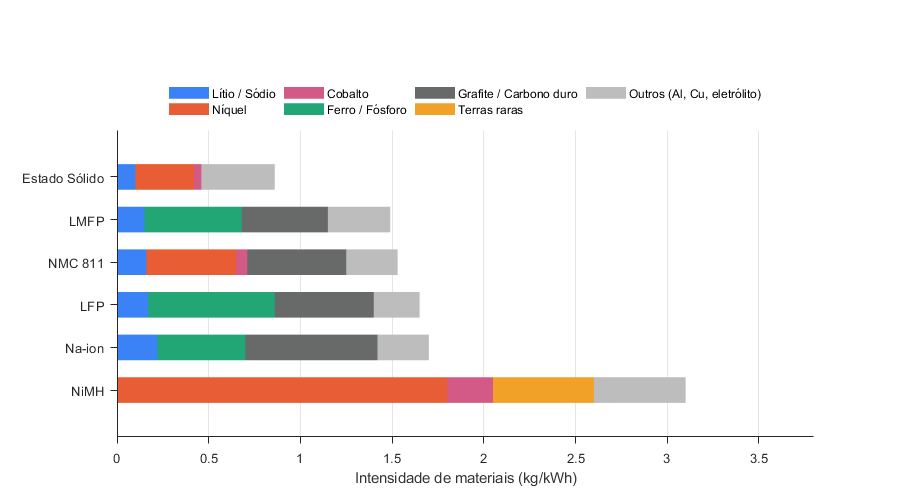
\includegraphics[width=\textwidth]{figuras/comparacao_quimica_baterias.png}
    \caption{Intensidade de materiais por tecnologia de bateria (kg por kWh).}
    \label{fig:intensidade-materiais}
    \fonte{elaborada com base em \citeonline{IEA2025} e \citeonline{McKinsey2026}.}
\end{figure}

\begin{table}[H]
\centering
\caption{Comparativo entre as tecnologias de bateria relevantes para a frota
         eletrificada brasileira.}
\label{tab:comparativo-quimicas}
\renewcommand{\arraystretch}{1.4}
\small
\begin{tabularx}{\textwidth}{@{} p{2.2cm} X X X @{}}
\toprule
\textbf{Tecnologia} & \textbf{Aspectos técnicos} &
\textbf{Dimensão econômica} & \textbf{Implicações para o fluxo de materiais} \\
\midrule
\textbf{NMC} &
Alta densidade energética; ideal para veículos de longa distância e
\textit{premium}. &
Custo elevado e volátil devido ao Co e ao Ni; foco em mercados maduros (UE/EUA). &
Alta dependência de minerais críticos com cadeias de suprimento instáveis; alto
valor de reciclagem. \\
\addlinespace
\textbf{LFP / LMFP} &
Alta segurança e longa vida útil; a evolução LMFP aumenta a densidade em até 20\%. &
Líder em custo-benefício (alvo de US\$~55--65/kWh); base da eletrificação de massa
no Brasil. &
Desafio na reciclagem: baixo valor dos materiais (Fe, P) dificulta a viabilidade
econômica sem escala. \\
\addlinespace
\textbf{NiMH} &
Alta densidade de potência e confiabilidade; limitada por menor densidade
energética; ideal para HEV. &
Tecnologia madura com custo consolidado; forte presença no Brasil via
híbridos-flex de alto volume. &
Elevado valor de reciclagem (Ni e terras raras); logística reversa economicamente
viável. \\
\addlinespace
\textbf{Na-ion} &
Menor densidade que o lítio; permite armazenamento com tensão zero, aumentando a
segurança logística. &
Tecnologia de reserva (\textit{backstop}) contra a volatilidade do lítio; paridade
de preço prevista para 2035. &
Abundância geográfica do sódio; reduz dependência de minerais escassos e o uso de
cobre. \\
\addlinespace
\textbf{Estado sólido} &
Fronteira tecnológica: densidade disruptiva (400+ Wh/kg) e recarga ultra-rápida
(12--20~min). &
Nicho de alto valor inicial; escala comercial projetada apenas para pós-2030 a
$\sim$US\$~100/kWh. &
Promete maior durabilidade (1.000--1.500 ciclos); fluxo de resíduos irrelevante no
horizonte desta pesquisa. \\
\bottomrule
\end{tabularx}
\fonte{elaborada pelos autores com base nas Seções~\ref{subsec:nmc} a~\ref{subsec:estadosolido}.}
\end{table}

% ===========================================================
\subsection{Manufatura de Células de Íon-Lítio}
\label{sec:manufatura}
% ===========================================================

A fabricação de células de íon-lítio organiza-se em três blocos de processo
\cite{knehr2022batpac,degen2022}: (i)~a produção de eletrodos — mistura dos
materiais ativos, aditivos condutores e aglutinantes em pasta, revestimento sobre
as folhas coletoras (alumínio no catodo, cobre no anodo), secagem com recuperação
do solvente e calandragem; (ii)~a montagem da célula — corte, empilhamento ou
enrolamento com o separador, inserção no invólucro e soldagem, em sala seca de
baixo ponto de orvalho, seguidas do enchimento com eletrólito e da selagem; e
(iii)~o acabamento — formação da interface sólido-eletrólito (SEI) por ciclos de
carga controlados, degasagem, envelhecimento e teste para classificação das
células.

Dois aspectos dessa cadeia são centrais para a análise de fluxos. O primeiro é a
geração de refugo em todas as etapas — pasta fora de especificação na mistura,
eletrodo revestido descartado no revestimento e no corte e células reprovadas na
formação e no teste —, de composição conhecida e homogênea, o que o diferencia das
baterias pós-consumo (Seção~\ref{subsec:lfp-economics}). O segundo é a
concentração do consumo de energia em operações que não transformam
quimicamente o material: a secagem dos eletrodos com recuperação do solvente
N-metil-2-pirrolidona (NMP), o controle de umidade da sala seca e a formação
respondem pela maior parte da energia da planta \cite{degen2022}. O
Capítulo~\ref{sec:gigafabrica} quantifica esses fluxos para uma fábrica de células
LFP.

% ===========================================================
\subsection{Reciclagem, Segunda Vida e Regulação}
\label{sec:reciclagem}
% ===========================================================

À medida que a frota eletrificada brasileira se expande, o destino das baterias ao
fim de sua vida útil torna-se mais urgente. A reciclagem de baterias de íon-lítio
(LIB) cumpre um papel duplo: resposta ambiental necessária para evitar a
contaminação por metais pesados e oportunidade estratégica de recuperação de
materiais críticos — lítio, cobalto, níquel e manganês — que realimentam a
produção de novas células. Esta seção apresenta as tecnologias de reciclagem,
analisa os desafios econômicos da química LFP, discute a segunda vida e
contextualiza o panorama regulatório.

\subsubsection{Pré-tratamento e Preparação das Células}
\label{subsec:pretratamento}

Independentemente da rota, as tecnologias de recuperação compartilham etapas de
pré-tratamento que determinam a eficiência, a segurança e o custo das fases
subsequentes \cite{latini2022apudhu2024}. A primeira é a descarga elétrica das
células, que devem ser reduzidas a uma tensão inferior a 1{,}5\,V antes de
qualquer manipulação mecânica. Na sequência, a trituração (\textit{shredding}), o
peneiramento e a separação por densidade produzem a \textit{black mass} —
mistura dos materiais ativos do catodo e do anodo com impurezas —, insumo central
das etapas piro e hidrometalúrgicas, cuja qualidade influencia diretamente a
eficiência da recuperação.

A logística reversa que antecede o pré-tratamento é ela própria um gargalo: em
revisão de 60 estudos, \citeonline{slattery2021} identificaram a coleta e o
transporte como desafio à reutilização ou à reciclagem em 70\% deles, e o
transporte respondeu, em média, por cerca de 41\% do custo total de reciclagem
nos estudos de custo analisados.

\subsubsection{Rotas de Reciclagem}
\label{subsec:rotas}

A literatura consolida cinco grandes rotas tecnológicas para a reciclagem de LIBs
\cite{biswal2024,balachandran2024}: pirometalurgia, hidrometalurgia, reciclagem
direta, biolixiviação e métodos eletroquímicos.

\paragraph{Pirometalurgia.}
Rota mais madura e amplamente implantada comercialmente (TRL~9). Consiste na fusão
das células ou da \textit{black mass} a \textbf{1.400--1.500\,°C}, produzindo uma
liga metálica rica em cobalto, níquel e cobre, posteriormente refinada por etapas
hidrometalúrgicas. Suas limitações incluem a perda de lítio e grafite para a
escória, a alta intensidade energética e a emissão de compostos fluorados da
decomposição do eletrólito (LiPF\textsubscript{6}). Para o LFP — cujo principal
elemento de valor, o lítio, é perdido na escória, e cujos ferro e fósforo têm
baixo valor de recuperação —, a adequação é baixa. Em termos climáticos, a revisão
de \citeonline{stegemann2025} indica que a combinação de rotas piro e
hidrometalúrgicas reduz em 27\% as emissões associadas à produção da célula.

\paragraph{Hidrometalurgia.}
Rota de maior presença na literatura — cerca de 57\% das publicações sobre
reciclagem de LIBs \cite{zhao2025}. Baseia-se na dissolução da \textit{black
mass} em soluções ácidas (clorídrico, sulfúrico ou nítrico), seguida de
purificação, precipitação seletiva e extração por solvente para separar lítio,
cobalto, níquel, manganês e cobre em compostos de alta pureza. Apresenta menor
intensidade energética ($<$100\,°C), recupera o lítio como carbonato ou hidróxido
de grau bateria ($>$90\% em meio ácido) e pode ser dimensionada para volumes
menores, o que a torna mais adequada a mercados emergentes como o Brasil.
\citeonline{stegemann2025} reportam redução de 39\% nas emissões da produção da
célula, com média de $-25{,}5$~kg\,CO\textsubscript{2}eq/kWh entre os estudos de
baterias NMC analisados — o melhor desempenho entre as rotas avaliadas na revisão.
Para o LFP, a viabilidade econômica permanece frágil, dado o baixo valor dos
materiais recuperados (Seção~\ref{subsec:lfp-economics}).

\paragraph{Reciclagem direta (\textit{direct recycling}).}
Visa \textbf{preservar e regenerar a estrutura cristalina} do material ativo do
cátodo, evitando a dissolução e a re-síntese química completa, por meio de
(i)~separação e coleta do material ativo, (ii)~relitiação e (iii)~tratamento
térmico para restaurar a ordem estrutural. O material regenerado pode ser usado
diretamente em novas baterias. \citeonline{balachandran2024} identificam essa rota
como a de maior potencial para a economia circular, mas com desafios de
homogeneidade dos lotes de entrada e de reprodutibilidade do desempenho
eletroquímico. Para o LFP, a estabilidade do LiFePO\textsubscript{4} facilita a
regeneração, e estudos recentes demonstraram a recuperação de
FePO\textsubscript{4} de resíduos de extração de lítio para uso em novas células
\cite{hu2024}. Maturidade atual: TRL~5--7.

\paragraph{Biolixiviação e métodos eletroquímicos.}
A biolixiviação utiliza microrganismos acidofílicos (principalmente
\textit{Acidithiobacillus thiooxidans} e \textit{A.~ferrooxidans}) para solubilizar
metais da \textit{black mass} com menor consumo de reagentes, mas ainda apresenta
taxas de extração mais baixas e tempos de processo mais longos (TRL~3--5)
\cite{balachandran2024}. Os métodos eletroquímicos recuperam seletivamente metais
de soluções de lixiviação, com alta seletividade iônica e compatibilidade com
fontes renováveis; hoje são usados sobretudo como etapas de purificação em fluxos
hidrometalúrgicos, com desenvolvimento industrial pleno projetado para o período
pós-2030 (TRL~4--6) \cite{zhu2024}. A Tabela~\ref{tab:rotas-reciclagem} sintetiza
as rotas.

\begin{table}[H]
\centering
\caption{Comparativo entre as rotas de reciclagem de baterias de íon-lítio.}
\label{tab:rotas-reciclagem}
\small
\renewcommand{\arraystretch}{1.2}
\begin{tabularx}{\textwidth}{@{} p{3cm} X X X X @{}}
\toprule
\textbf{Critério} & \textbf{Pirometalurgia} & \textbf{Hidrometalurgia} &
\textbf{Reciclagem Direta} & \textbf{Bio / Eletroquímica} \\
\midrule
Maturidade (TRL) & Alta (TRL~9) — comercial & Alta (TRL~9) — comercial &
Média (TRL~5--7) — piloto & Baixa/Média (TRL~3--6) — laboratório \\
\addlinespace
Temperatura & 1.400--1.500\,°C & $<$100\,°C & 200--900\,°C (recozimento) &
Ambiente ($\sim$25--50\,°C) \\
\addlinespace
Recuperação de Li & Muito baixa (Li vai para a escória) &
Alta ($>$90\% em meio ácido) & Alta (com relitiação) & Moderada a alta \\
\addlinespace
Adequação ao LFP & Baixa — Li perdido na escória; Fe e P sem valorização &
Moderada — rentabilidade limitada & Alta — estrutura olivínica estável &
Em avaliação \\
\addlinespace
Impacto climático$^{a}$ & $-$27\% (rotas piro e hidro combinadas) &
$-$39\% & Potencialmente inferior ao hidro & Em estudo \\
\addlinespace
Custo relativo & Alto (\textit{capex} elevado, escala de fusão) &
Médio (reagentes + efluentes) & Baixo/Médio (dependente de escala) &
Baixo (perspectiva de longo prazo) \\
\bottomrule
\end{tabularx}
\par\vspace{2pt}{\footnotesize $^{a}$Redução das emissões em relação à produção
da célula \cite{stegemann2025}.}
\fonte{adaptado de \citeonline{balachandran2024} e \citeonline{stegemann2025}.}
\end{table}

\subsubsection{Desafios Econômicos da Reciclagem do LFP}
\label{subsec:lfp-economics}

A predominância de baterias LFP na frota eletrificada brasileira coloca o país
diante de uma dificuldade estrutural de reciclagem. Ao contrário das baterias NMC,
que contêm cobalto e níquel em proporções significativas, os componentes do LFP
(lítio, ferro e fósforo) possuem valor intrínseco substancialmente menor. O valor
de mercado dos materiais recuperados de baterias LFP situa-se entre USD~300 e
USD~600 por tonelada \pendente{indicar a fonte original; o valor não consta de
\citeonline{stegemann2025}}, o que resulta em prejuízo líquido sob as condições
operacionais atuais da maior parte das instalações. Os recicladores tendem a
priorizar materiais críticos de maior valor, e as baterias LFP são menos propensas
a ser recicladas \cite{nrel2023}.

Esse cenário é agravado pela queda do preço do carbonato de lítio — que recuou de
picos históricos em 2022 para valores muito inferiores em 2024--2025 —, que reduz o
incentivo à recuperação do lítio. \citeonline{chen2025} identificam gargalos
adicionais: a estabilidade da estrutura olivínica do LiFePO\textsubscript{4} exige
condições ácidas mais agressivas de lixiviação; o ferro e o fósforo não possuem
rotas de valorização simples nas cadeias existentes; e normas crescentes sobre
efluentes ácidos e resíduos fluorados elevam os custos de conformidade. Somente
grandes volumes reduzem o custo unitário ao ponto de rentabilidade; no Brasil, o
momento em que os volumes de fim de vida atingirão essa escala depende do MFA
dinâmico da frota, indicado como continuidade deste trabalho
(Capítulo~\ref{sec:conclusao}).

A resposta tecnológica mais promissora é a reciclagem direta do material ativo
do catodo LFP, que elimina a dissolução e a re-síntese química completa;
complementarmente, a recuperação de grafite, inclusive a partir de baterias LFP,
pode melhorar a economia do processo \cite{nrel2023}. Nesse contexto, a sucata de
produção — homogênea, de composição conhecida e livre de contaminação — tende a
ser economicamente mais atrativa do que o material pós-consumo e é quantificada
no Capítulo~\ref{sec:gigafabrica}. A Tabela~\ref{tab:lfp-gargalos} sintetiza
esses gargalos.

\begin{table}[H]
\centering
\caption{Gargalos econômicos da reciclagem de baterias LFP e implicações para o
         contexto brasileiro.}
\label{tab:lfp-gargalos}
\small
\renewcommand{\arraystretch}{1.2}
\begin{tabularx}{\textwidth}{@{} p{3cm} X X @{}}
\toprule
\textbf{Fator} & \textbf{Descrição} & \textbf{Implicação para o Brasil} \\
\midrule
Baixo valor intrínseco dos materiais &
Fe e P têm valor de mercado muito inferior ao Co e ao Ni do NMC &
Margens negativas nas operações convencionais; recicladores priorizam
materiais de maior valor \\
\addlinespace
Queda do preço do carbonato de lítio &
Pico histórico em 2022; recuo acentuado em 2024--2025 reduz o valor do Li
recuperado &
Diminui o único componente de valor relativo do LFP, piorando a equação econômica \\
\addlinespace
Dificuldade de lixiviação seletiva &
Estrutura olivínica estável exige condições ácidas mais agressivas, elevando o
custo de reagentes &
Aumenta o custo operacional da hidrometalurgia aplicada ao LFP \\
\addlinespace
Baixa separabilidade de Fe e P &
Ferro e fósforo não possuem rotas de valorização simples nas cadeias existentes &
Limita receitas secundárias e onera o tratamento de efluentes \\
\addlinespace
Escala insuficiente (curto prazo) &
Apenas grandes volumes reduzem o custo unitário ao ponto de rentabilidade &
Momento de atingir escala depende dos volumes de fim de vida da frota (MFA
dinâmico, etapa futura); a sucata de produção pode antecipar parte dessa escala \\
\bottomrule
\end{tabularx}
\fonte{elaborada com base em \citeonline{chen2025} e \citeonline{nrel2023}.}
\end{table}

\subsubsection{Segunda Vida das Baterias (\textit{Second-Life})}
\label{subsec:secondlife}

Uma etapa intermediária de grande relevância estratégica — tanto para ampliar o
valor econômico extraído das baterias quanto para aliviar a pressão sobre a
infraestrutura de reciclagem — é a reutilização em \textbf{aplicações de segunda
vida} (\textit{second-life batteries}, SLB). Ao fim da vida útil veicular — quando
a capacidade remanescente cai abaixo do limiar adequado à tração
\pendente{informar o limiar adotado, em \% da capacidade inicial, e a fonte} —, a
bateria ainda retém capacidade suficiente para aplicações estacionárias de menor
exigência \cite{moseley2019}, como armazenamento de energia em edifícios,
subestações de fontes renováveis e infraestrutura de telecomunicações.

\citeonline{baars2021} indicam que o reaproveitamento pode satisfazer mais de
100\% da demanda de armazenamento estacionário por baterias de segunda vida até
2050, enquanto a reciclagem cobriria cerca de 61\% da demanda por materiais de
novas baterias no mesmo período \cite{est2025}. A segunda vida posterga o ingresso
das baterias no sistema de reciclagem por 8 a 12 anos após o fim do uso veicular
\cite{mdpisustain2024}; para baterias LFP, de maior longevidade em ciclos, essa
janela pode ser ainda mais extensa.

A implantação de mercados de segunda vida enfrenta barreiras de padronização da
avaliação do estado de saúde (\textit{State of Health} — SOH), de classificação
regulatória das baterias retiradas — frequentemente tratadas como resíduo
perigoso, o que dificulta transporte e comercialização —, de responsabilidade
legal e garantias de desempenho e de modelos de negócio que conectem
desmontadores, certificadores e operadores de armazenamento \cite{moseley2019}.
Para o Brasil, a regulamentação da segunda vida deve integrar uma política
nacional de baterias; o volume de baterias LFP e NiMH aptas ao reaproveitamento e
o momento em que esse volume se tornará relevante dependem do MFA dinâmico da
frota (Capítulo~\ref{sec:conclusao}).

\subsubsection{Contexto Regulatório: Brasil e Panorama Internacional}
\label{subsec:regulatorio}

A maturidade do ecossistema de reciclagem de baterias está diretamente atrelada à
solidez do arcabouço regulatório. A literatura identifica um gradiente que vai da
China e da União Europeia — referências globais — até economias emergentes como o
Brasil, cujo quadro normativo permanece fragmentado \cite{regulationsmdpi2025}.

Na China, desde 2016 consolida-se um arcabouço de Responsabilidade Estendida do
Produtor (EPR) com rastreabilidade digital (passaporte de bateria), metas de
coleta e reciclagem atribuídas aos fabricantes de veículos e incentivos fiscais a
recicladores certificados; a taxa de reciclagem de baterias de veículos elétricos
elevou-se de 25\% em 2020 para 40\% em 2023 \cite{miit2024}. Na União Europeia, o
Regulamento (UE) 2023/1542 estabelece metas de coleta e de eficiência de
reciclagem e exige passaporte digital para baterias de veículos elétricos a
partir de 18 de fevereiro de 2027 \cite{eu2023battery}. A Coreia do Sul, desde
2024, classifica as baterias de veículos elétricos como ``recursos recicláveis'',
desonerando unidades não danificadas das regras de resíduos perigosos, e prevê
avaliação obrigatória de desempenho antes da retirada do veículo a partir de 2027
\cite{regulationsmdpi2025}.

No Brasil, a Política Nacional de Resíduos Sólidos (Lei 12.305/2010) estabelece o
princípio da responsabilidade compartilhada e obriga a logística reversa de
pilhas e baterias \cite{pnrs2010}, mas não foi adaptada às especificidades das
baterias de tração. A Resolução CONAMA 401/2008, que revogou a Resolução
257/1999, estabelece limites de chumbo, cádmio e mercúrio para pilhas e baterias
e critérios para seu gerenciamento ambientalmente adequado, sem tratar
especificamente das baterias de íon-lítio de veículos elétricos
\cite{conama2008,oliveira2025}. Em 6 de maio de 2025, foi apresentado no Senado
Federal o PL 2.132/2025, que institui a Política Nacional de Circularidade das
Baterias Veiculares, com passaporte de bateria contendo dados de composição,
origem e possibilidades de reuso, além de metas de rastreabilidade e
circularidade a serem definidas pelo governo \cite{dialogueearth2026}
\pendente{confirmar a situação regulatória vigente na data de entrega do
relatório}.

O Brasil possui uma referência de sucesso que pode orientar essa construção: o
sistema de reciclagem de baterias de chumbo-ácido (ULABs), que, por meio de
certificação INMETRO, eliminação de impostos sobre sucata e responsabilidade
compartilhada, transicionou para um modelo formalizado e ambientalmente
responsável \cite{leadbatteries2024}.

\begin{table}[H]
\centering
\caption{Comparativo do contexto regulatório para reciclagem de baterias de VE.}
\label{tab:regulatorio}
\small
\renewcommand{\arraystretch}{1.2}
\begin{tabularx}{\textwidth}{@{} p{2.6cm} X X X @{}}
\toprule
\textbf{Dimensão} & \textbf{China} & \textbf{UE / Coreia do Sul} & \textbf{Brasil} \\
\midrule
Modelo regulatório &
EPR com metas obrigatórias (desde 2016) &
Regulamento (UE) 2023/1542: passaporte digital, metas de coleta e de eficiência
de reciclagem &
PNRS (2010), Resolução CONAMA 401/2008 e legislações estaduais (SP, MG); sem
marco específico para baterias de tração \\
\addlinespace
Rastreabilidade &
Passaporte de bateria digital obrigatório; plataforma governamental de
monitoramento &
Passaporte digital obrigatório a partir de 18/02/2027 (UE) &
PL 2.132/2025, apresentado em maio de 2025, prevê passaporte; em tramitação \\
\addlinespace
Taxa de reciclagem &
25\% (2020) $\to$ 40\% (2023); meta de 70\% até 2027 &
Metas de 70--80\% em peso por química até 2030; Coreia do Sul: baterias de VE
como ``recursos recicláveis'' desde 2024 &
Sem metas quantitativas definidas para baterias de tração \\
\addlinespace
Referência de sucesso &
Sistema nacional integrado com incentivos fiscais e certificação de recicladores &
Modelo de passaporte digital como referência global &
Sistema ULAB (baterias de chumbo-ácido): modelo a replicar \\
\bottomrule
\end{tabularx}
\fonte{elaborada com base em \citeonline{regulationsmdpi2025},
       \citeonline{eu2023battery}, \citeonline{conama2008},
       \citeonline{oliveira2025} e \citeonline{dialogueearth2026}.}
\end{table}

\subsubsection{Síntese: Implicações para a Cadeia Nacional de Reciclagem}
\label{subsec:sintese-reciclagem}

A análise das rotas de reciclagem revela que não existe solução única e
universalmente ótima para o contexto brasileiro. O caminho mais adequado à
composição da frota nacional combina três elementos complementares:

\begin{enumerate}
    \item \textbf{Aposta na reciclagem direta e na hidrometalurgia eficiente para o
    LFP}, que apresentam melhor equilíbrio entre recuperação de lítio e custo
    operacional;

    \item \textbf{Desenvolvimento do mercado de segunda vida} para baterias LFP e
    NiMH, postergando a entrada na cadeia de reciclagem e gerando valor
    intermediário alinhado à expansão das renováveis na matriz elétrica;

    \item \textbf{Construção de arcabouço regulatório} específico para baterias de
    tração, com instrumentos de EPR, rastreabilidade e incentivos à coleta e à
    reciclagem locais, aproveitando as lições do sistema de baterias de
    chumbo-ácido.
\end{enumerate}

Sem volume suficiente de material processado, nenhuma rota tecnológica alcança
rentabilidade. Dois fluxos alimentarão uma cadeia nacional: a sucata de produção,
homogênea e disponível desde o início da fabricação de células, quantificada no
Capítulo~\ref{sec:gigafabrica}, e as baterias pós-consumo, cujos volumes e
cronologia dependem do MFA dinâmico da frota, indicado como continuidade deste
trabalho.

\newpage
\section{Resultados: \textit{Market Share} e Cenários de Frota}
\label{sec:resultados}

% ===========================================================
\subsection{Market Share de Químicas de Baterias}
\label{sec:marketshare}
% ===========================================================

Determinar a participação de mercado (\textit{market share}) das diferentes
químicas de baterias em circulação no Brasil é uma etapa fundamental para
caracterizar a frota eletrificada e orientar a escolha da química do estudo
industrial. Para isso, o levantamento baseou-se no cruzamento de dados de
emplacamentos de veículos eletrificados, fornecidos pela Associação Brasileira do
Veículo Elétrico (ABVE), com as especificações técnicas do Programa Brasileiro de
Etiquetagem Veicular (PBEV), conforme descrito na Seção~\ref{sec:met-marketshare}.

A partir da consolidação desses dados, que englobou uma amostra de mais de
509~mil veículos eletrificados, foi possível estimar a participação de cada
tecnologia de bateria nos emplacamentos. As participações são calculadas em número
de veículos; por isso, refletem a frequência de cada química, e não sua
participação em massa ou em capacidade. Os resultados revelam uma configuração de
mercado particular, moldada pela predominância de modelos de entrada e híbridos.

A química de Lítio-Ferro-Fosfato (LFP) representa \textbf{48,12\%} dos veículos
analisados. Esse domínio reflete a forte penetração de montadoras asiáticas no
Brasil, que priorizam o LFP para reduzir o custo final ao consumidor e viabilizar
a comercialização de veículos elétricos e híbridos \textit{plug-in}.

Em segundo lugar, as baterias baseadas em Níquel-Manganês-Cobalto (NMC) respondem
por \textbf{32,75\%} da amostra. Sua aplicação concentra-se em veículos que
demandam maior densidade energética, como modelos de alta performance e híbridos
\textit{plug-in} de categorias superiores.

Destaca-se também a participação expressiva das baterias NiMH (níquel-metal
hidreto), que compõem \textbf{18,38\%} da amostra. Esse volume é sustentado quase
exclusivamente pelos híbridos convencionais (HEV) da Toyota. Tecnologias
minoritárias — NCMA (0,52\%), LMO/NMC (0,15\%) e variações de íon-lítio ainda em
confirmação (0,08\%) — somam juntas menos de 1\% do total, conforme sintetizado na
Tabela~\ref{tab:marketshare-sintese} e ilustrado na Figura~\ref{fig:marketshare}.

\begin{table}[H]
\centering
\caption{Síntese do \textit{market share} por química de bateria nos veículos
         eletrificados emplacados (participação em número de veículos).}
\label{tab:marketshare-sintese}
\begin{tabular}{lc}
\toprule
\textbf{Química da Bateria} & \textbf{Market Share} \\
\midrule
LFP (Lítio-Ferro-Fosfato)                          & 48,12\% \\
NMC (Níquel-Manganês-Cobalto)                      & 32,75\% \\
NiMH (Níquel-Metal Hidreto)                        & 18,38\% \\
NCMA (Níquel-Cobalto-Manganês-Alumínio)            &  0,52\% \\
LMO/NMC (Óxido de Manganês / Níquel-Mang.-Cobalto) &  0,15\% \\
Lítio-Íon (a confirmar)                            &  0,08\% \\
\bottomrule
\end{tabular}
\fonte{elaborada com base em \citeonline{ABVE} e \citeonline{PBEV}.}
\end{table}

\begin{figure}[H]
    \centering
    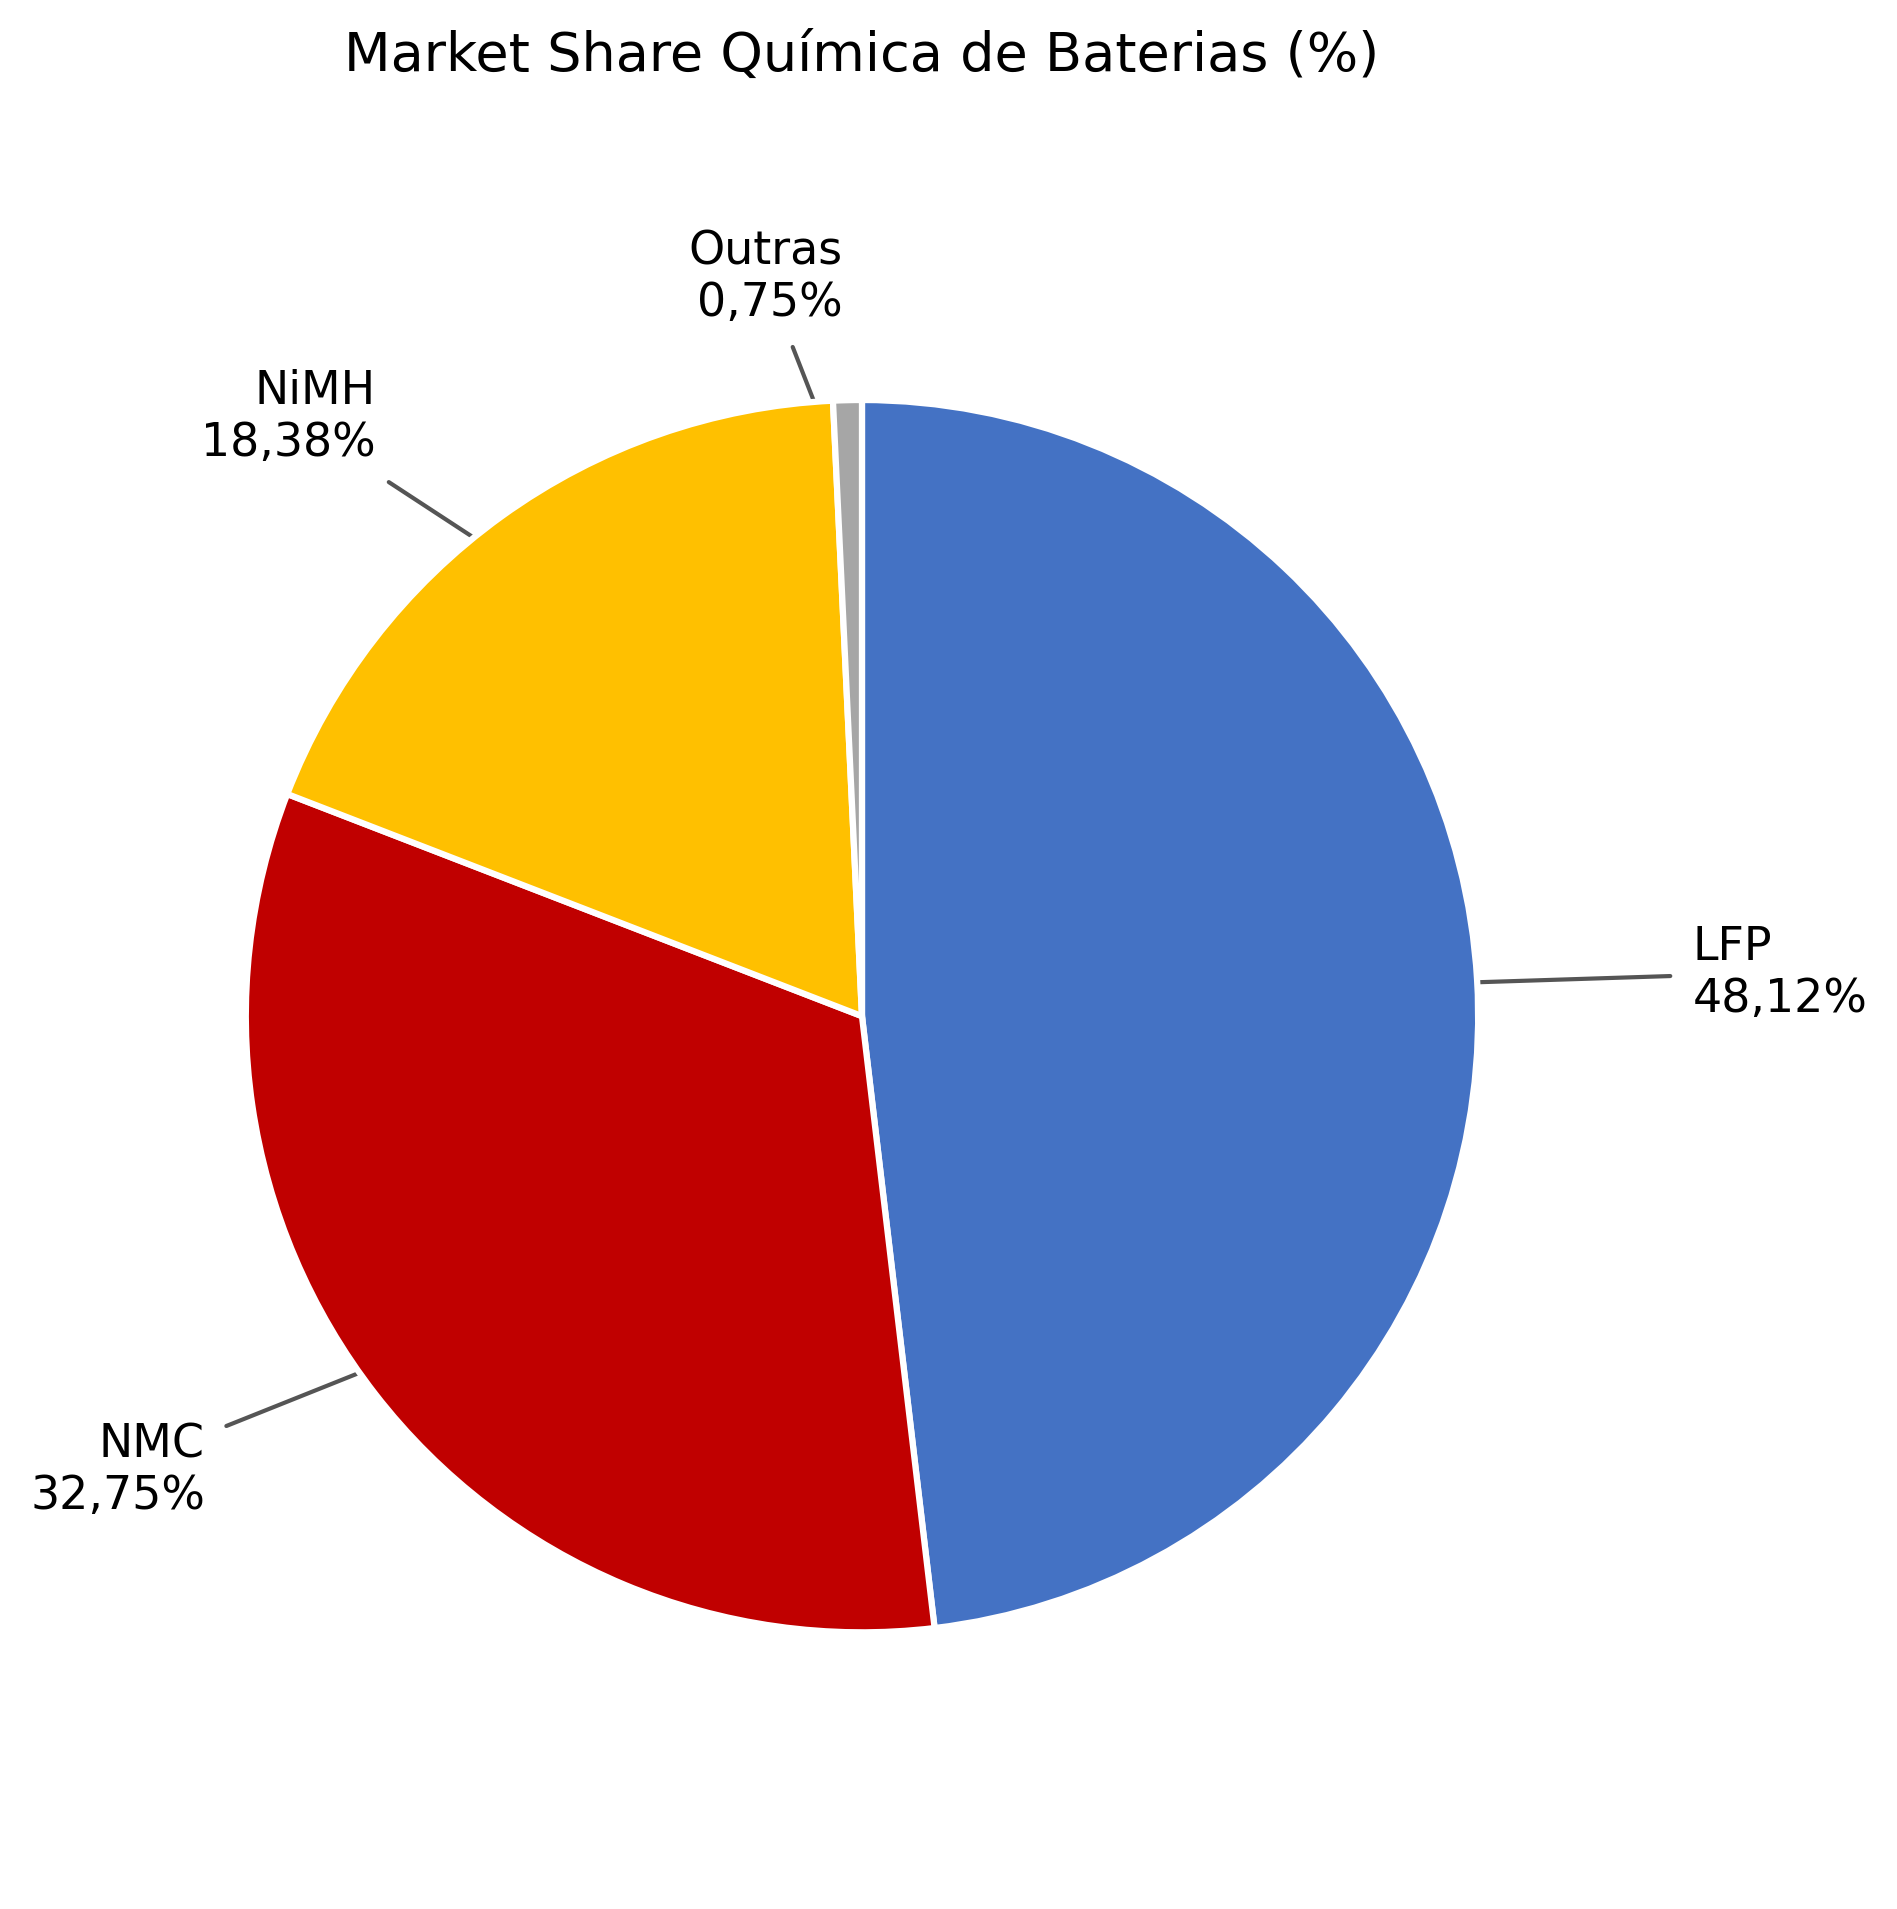
\includegraphics[width=0.6\textwidth]{figuras/market_share_quimicas.png}
    \caption{Participação das químicas de bateria nos veículos eletrificados
             emplacados (em número de veículos).}
    \label{fig:marketshare}
    \fonte{elaborada com base em \citeonline{ABVE} e \citeonline{PBEV}.}
\end{figure}

Este panorama estabelece a linha de base da composição química da frota
eletrificada. A predominância de químicas isentas de cobalto e níquel (como o LFP)
na maior parcela dos veículos indica que o futuro brasileiro terá uma concentração
expressiva de ferro, fósforo e lítio nas baterias em circulação, reforçando a
premissa de que a reciclagem no país exigirá processos eficientes, focados em
ganho de escala.

\subsubsection{Base de Dados de Emplacamentos}
\label{subsec:emplacamentos}

A Tabela~\ref{tab:emplacamentos-geral} apresenta os 15 modelos eletrificados de
maior volume de vendas (todas as categorias combinadas), com a química de bateria
atribuída a cada um. As participações por modelo são calculadas sobre o total de
emplacamentos da base — cerca de 593~mil veículos, valor implícito na própria
tabela (51.551 / 8,69\%) —, e não sobre a amostra de 509~mil veículos com química
identificada utilizada na Tabela~\ref{tab:marketshare-sintese}
\pendente{confirmar os dois denominadores na planilha-fonte e o número de modelos
da amostra geral: a nota da tabela cita 50 modelos, e as
Tabelas~\ref{tab:bev} e~\ref{tab:hev} listam 49 BEV e 21 HEV}.

\begin{table}[H]
\centering
\caption{Modelos eletrificados de maior volume de emplacamento (geral) e química
         de bateria associada.}
\label{tab:emplacamentos-geral}
\begin{tabular}{lccc}
\toprule
\textbf{Modelo} & \textbf{Quantidade} & \textbf{Market Share} & \textbf{Química} \\
\midrule
Toyota Corolla Cross XRX Hybrid & 51.551 & 8,69\% & NiMH \\
BYD Dolphin Mini GS5 EV         & 44.730 & 7,54\% & LFP \\
BYD Song Plus GS DM             & 44.652 & 7,53\% & LFP \\
BYD Dolphin GS 180 EV           & 32.334 & 5,45\% & LFP \\
BYD Song Pro GS DM              & 30.274 & 5,11\% & LFP \\
Toyota Corolla Altis Premium H  & 22.147 & 3,73\% & NiMH \\
GWM Haval H6 PHEV 19            & 16.946 & 2,86\% & NMC \\
BYD Dolphin Mini GS EV          & 15.820 & 2,67\% & LFP \\
GWM Haval H6 Premium HEV        & 15.623 & 2,63\% & NMC \\
BYD King GS DM                  & 15.181 & 2,56\% & LFP \\
GWM Haval H6 GT                 & 13.088 & 2,21\% & NMC \\
GWM Haval H6 Premium PHEV       & 10.911 & 1,84\% & NMC \\
CAOA Chery Tiggo 8 PHEV         &  9.759 & 1,65\% & NMC \\
BYD Seal AWD GS 590 EV          &  8.132 & 1,37\% & LFP \\
BYD Dolphin Plus 310 EV         &  7.631 & 1,29\% & LFP \\
\bottomrule
\end{tabular}
\fonte{elaborada com base em \citeonline{ABVE} e \citeonline{PBEV}.}
\end{table}

\subsubsection{Composição por Categoria de Veículo}
\label{subsec:composicao-categoria}

Segmentando a amostra por categoria de veículo, observa-se que a predominância do
LFP concentra-se nos modelos 100\% elétricos (BEV) — nove dos doze modelos da
Tabela~\ref{tab:bev} utilizam LFP —, enquanto o NiMH está associado quase
exclusivamente aos híbridos convencionais (HEV) da Toyota; o Honda Civic Hybrid
da amostra utiliza bateria de íon-lítio. Não foi possível isolar, na base de dados
consultada, uma quebra específica para a categoria de híbridos \textit{plug-in}
(PHEV): os modelos dessa categoria permanecem diluídos no levantamento agregado da
Tabela~\ref{tab:emplacamentos-geral} (por exemplo, GWM Haval H6 PHEV, CAOA Chery
Tiggo 8 PHEV e GWM Tank 300 PHEV), motivo pelo qual a segmentação apresentada a
seguir limita-se às categorias BEV e HEV.

\begin{table}[H]
\centering
\caption{Composição química — veículos 100\% elétricos (BEV), modelos mais
         relevantes.}
\label{tab:bev}
\begin{tabular}{lccc}
\toprule
\textbf{Modelo} & \textbf{Quantidade} & \textbf{Market Share (BEV)} & \textbf{Química} \\
\midrule
BYD Dolphin Mini GS5 EV  & 44.730 & 23,98\% & LFP \\
BYD Dolphin GS 180 EV    & 32.334 & 17,34\% & LFP \\
BYD Dolphin Mini GS EV   & 15.820 &  8,48\% & LFP \\
BYD Seal AWD GS 590 EV   &  8.132 &  4,36\% & LFP \\
BYD Dolphin Plus 310 EV  &  7.631 &  4,09\% & LFP \\
BYD Yuan Pro GS 290 EV   &  6.344 &  3,40\% & LFP \\
GWM Ora 03 Skin BEV48    &  5.780 &  3,10\% & LFP \\
BYD Yuan Plus GL 310 EV  &  5.390 &  2,89\% & LFP \\
GWM Ora 03 GT BEV63      &  4.305 &  2,31\% & NMC \\
Volvo EX30 E60 Ultra     &  3.275 &  1,76\% & NMC \\
Renault E-Kwid Intens    &  3.061 &  1,64\% & NMC \\
JAC E-JS1                &  2.872 &  1,54\% & LFP \\
\bottomrule
\end{tabular}
\fonte{elaborada com base em \citeonline{ABVE} e \citeonline{PBEV}. Amostra
       completa de 49 modelos (172.384 unidades, $\sim$92,4\% da categoria BEV).}
\end{table}

\begin{table}[H]
\centering
\caption{Composição química — híbridos convencionais (HEV), modelos mais
         relevantes.}
\label{tab:hev}
\begin{tabular}{lccc}
\toprule
\textbf{Modelo} & \textbf{Quantidade} & \textbf{Market Share (HEV)} & \textbf{Química} \\
\midrule
Toyota Corolla Cross XRX Hybrid & 51.551 & 34,91\% & NiMH \\
Toyota Corolla Altis Premium H  & 22.147 & 15,00\% & NiMH \\
GWM Haval H6 Premium HEV        & 15.623 & 10,58\% & NMC \\
Toyota RAV4 H SX AWD CNT        &  6.895 &  4,67\% & NiMH \\
GWM Haval H6 HEV                &  5.689 &  3,85\% & NMC \\
Toyota Corolla Cross XRV Hybrid &  5.367 &  3,63\% & NiMH \\
GWM Haval H6 HEV2               &  3.779 &  2,56\% & NMC \\
Toyota Corolla GLI HEV          &  3.503 &  2,37\% & NiMH \\
CAOA Chery Tiggo 7 Pro HA       &  3.340 &  2,26\% & NMC \\
Toyota Corolla Altis HV         &  3.298 &  2,23\% & NiMH \\
Honda Civic Hybrid Touring      &  3.265 &  2,21\% & Li-Ion (NMC) \\
\bottomrule
\end{tabular}
\fonte{elaborada com base em \citeonline{ABVE} e \citeonline{PBEV}. Amostra
       completa de 21 modelos (140.517 unidades, $\sim$95,1\% da categoria HEV).}
\end{table}

% ===========================================================
\subsection{Cenários de Frota}
\label{sec:cenarios-frota}
% ===========================================================

Para estabelecer as projeções de eletrificação da frota automotiva brasileira com
horizontes em 2030, 2035 e 2040, conforme descrito na
Seção~\ref{sec:met-cenarios}, foram sintetizadas as projeções de quatro fontes
institucionais: estudo ANFAVEA/BCG, PDE~2035 (EPE/MME), Bright Consulting e MBC
Brasil.

\subsubsection{Veículos Leves}
\label{subsec:leves}

Antes de discutir os cenários, é importante situar o peso de cada categoria na
massa de baterias, já que a análise de fluxo de materiais depende não apenas do
número de veículos, mas sobretudo da massa de bateria que cada categoria introduz
no sistema. A Tabela~\ref{tab:categoria-massa} combina o \textit{mix} de vendas de
eletrificados projetado pelo PDE~2035 para 2035 — 13\% HEV, 3,5\% PHEV e 6\% BEV
das vendas totais de veículos leves \cite{EPE2025}, ou 57,8\%, 15,6\% e 26,7\% das
vendas de eletrificados — com massas médias de pacote adotadas como hipótese.

\begin{table}[H]
\centering
\caption{Participação de cada categoria nas vendas de eletrificados (PDE~2035) e
         na massa de baterias vendidas.}
\label{tab:categoria-massa}
\small
\setlength{\tabcolsep}{5pt}
\begin{tabular}{lccc}
\toprule
\textbf{Categoria} & \textbf{Vendas de eletrificados} & \textbf{Massa média do pacote (H)} &
\textbf{Massa de baterias vendidas} \\
\midrule
HEV  & 57,8\% & $\sim$40\,kg  & 14,1\% \\
PHEV & 15,6\% & $\sim$130\,kg & 12,4\% \\
BEV  & 26,7\% & $\sim$450\,kg & 73,5\% \\
\bottomrule
\end{tabular}
\fonte{elaborada com base no \textit{mix} de vendas de \citeonline{EPE2025}; massas
       médias de pacote: hipótese deste trabalho \pendente{indicar a fonte das massas
       médias de pacote}.}
\end{table}

O contraste entre as colunas da Tabela~\ref{tab:categoria-massa} é revelador:
embora o HEV responda pela maior parte das vendas de eletrificados (57,8\%), sua
contribuição para a massa de baterias vendidas é pequena (14,1\%), dado o pacote
reduzido. Já o BEV, com pouco mais de um quarto das vendas, concentra cerca de
três quartos (73,5\%) da massa de bateria que entrará futuramente no fluxo de
reciclagem. A conclusão é robusta às massas adotadas: variações de $\pm$30\% na
massa média do pacote BEV mantêm sua participação entre 66\% e 78\%. Essa
constatação reforça a necessidade de tratar a análise de fluxo de materiais em
base mássica, e não apenas em número de veículos, sob pena de subestimar
sistematicamente a demanda por lítio e demais materiais críticos.

As projeções institucionais convergem para uma rota distinta das dos mercados
europeu e chinês, com prioridade à hibridização, sobretudo ao Híbrido-Flex
(Seção~\ref{subsec:contexto-brasil}). A Tabela~\ref{tab:projecoes-fontes}
consolida as projeções das quatro fontes analisadas.

\begin{table}[H]
\centering
\caption{Comparativo das projeções de eletrificação por fonte.}
\label{tab:projecoes-fontes}
\small
\renewcommand{\arraystretch}{1.2}
\setlength{\tabcolsep}{4pt}
\begin{tabularx}{\textwidth}{@{} >{\raggedright\arraybackslash}p{2.5cm} >{\raggedright\arraybackslash}p{1.7cm} >{\raggedright\arraybackslash}p{2.0cm} X X @{}}
\toprule
\textbf{Fonte} & \textbf{Horizonte} & \textbf{Métrica} &
\textbf{Dados projetados} & \textbf{Premissa principal} \\
\midrule
ANFAVEA/\allowbreak BCG & 2030--2040 & Frota circulante (leves) &
Eletrificados: 35\% (transição gradual) e 42\% (transição acelerada) em 2040;
detalhamento na Tabela~\ref{tab:bcg} &
Transição gradual com Híbrido-Flex \textit{vs.} transição acelerada com maior
penetração de \textit{plug-ins} \\
\addlinespace
Bright Consulting & 2030 & Frota circulante &
$\sim$9,8\% híbridos (HEV/PHEV); $\sim$1,9\% elétricos puros (BEV); total
eletrificado $\sim$6,5--7 milhões \pendente{conferir na fonte} &
Eletrificação total (BEV) limitada por custo e infraestrutura; aposta de massa no
Híbrido-Flex \\
\addlinespace
PDE 2035 & 2035 & Vendas (licenciamento) &
22,5--23\% de participação de mercado anual; \textit{mix}: 13\% HEV, 3,5\% PHEV,
6\% BEV &
Preferência por híbridos que aproveitam a infraestrutura de abastecimento
existente \\
\addlinespace
PDE 2035 & 2035 & Frota circulante &
3,7 milhões de veículos eletrificados (8\% da frota total) &
Renovação de frota lenta; combustão/flex ainda 87\% da frota
\pendente{conferir: 8\% + 87\% = 95\%} \\
\addlinespace
MBC Brasil & 2040 & Frota circulante &
17,4 milhões de veículos eletrificados (27\% da frota total); 72\% dos
eletrificados híbridos &
Crescimento exponencial (44$\times$ até 2040) \\
\bottomrule
\end{tabularx}
\fonte{elaborada com base em \citeonline{anfaveabcg2024},
       \citeonline{BrightConsulting}, \citeonline{EPE2025} e
       \citeonline{MBCBrasil}.}
\end{table}

O estudo ANFAVEA/BCG trabalha com dois cenários principais de eletrificação:
\textbf{transição gradual} (conservadora, com aposta no Híbrido-Flex) e
\textbf{transição acelerada} (otimista, com maior penetração de
\textit{plug-ins}). A Tabela~\ref{tab:bcg} detalha a projeção da frota de veículos
leves por motorização para os três horizontes analisados.

\begin{table}[H]
\centering
\caption{Projeção da frota de veículos leves por motorização — estudo
         ANFAVEA/BCG (milhões de veículos).}
\label{tab:bcg}
\small
\setlength{\tabcolsep}{4.5pt}
\begin{tabular}{llccccccc}
\toprule
\textbf{Ano} & \textbf{Cenário} & \textbf{Frota total} & \textbf{BEV} &
\textbf{PHEV} & \textbf{HEV} & \textbf{MHEV} & \textbf{ICE/Flex} &
\textbf{Eletrificados (\%)} \\
\midrule
\multirow{2}{*}{2030} & Gradual   & 52 & 1  & 1 & 1 & 2 & 48 & 9  \\
                      & Acelerada & 52 & 2  & 1 & 1 & 2 & 47 & 10 \\
\addlinespace
\multirow{2}{*}{2035} & Gradual   & 60 & 4  & 1 & 3 & 4 & 48 & 20 \\
                      & Acelerada & 60 & 5  & 1 & 4 & 4 & 44 & 25 \\
\addlinespace
\multirow{2}{*}{2040} & Gradual   & 71 & 9  & 2 & 7 & 8 & 48 & 35 \\
                      & Acelerada & 71 & 12 & 2 & 8 & 6 & 42 & 42 \\
\bottomrule
\end{tabular}
\fonte{\citeonline{anfaveabcg2024}. Valores arredondados ao milhão; por isso, a
       soma das categorias difere da frota total em até 2 milhões, exceto em 2040
       (transição gradual), em que as categorias somam 74 milhões para uma frota
       de 71 milhões \pendente{conferir no relatório completo ANFAVEA/BCG, que
       também deve ser citado para os valores de 2030 e 2035}.}
\end{table}

As Figuras~\ref{fig:comparacao-frotas} e~\ref{fig:composicao-frota} comparam,
respectivamente, os volumes absolutos e a composição percentual da frota projetada
por cada fonte, sempre no horizonte de cada projeção.

\begin{figure}[H]
\centering
\begin{tikzpicture}
\begin{axis}[
    ybar,
    bar width = 10pt,
    width  = 14.5cm,
    height = 7.2cm,
    symbolic x coords = {2030,2035,2040},
    xtick = data,
    enlarge x limits = 0.25,
    ymin = 0, ymax = 32,
    ylabel = {Frota eletrificada (milhões de veículos)},
    ylabel style = {font=\footnotesize},
    ticklabel style = {font=\footnotesize},
    ymajorgrids = true,
    grid style = {dotted, gray!40},
    axis x line* = bottom,
    axis y line* = left,
    nodes near coords,
    nodes near coords style = {font=\scriptsize},
    every node near coord/.append style = {/pgf/number format/use comma},
    legend style = {at={(0.5,-0.16)}, anchor=north, legend columns=3,
                    font=\footnotesize, draw=none, column sep=8pt},
    legend cell align = left,
]
\addplot[fill=gigaVerde!45, draw=black!60] coordinates {(2030,5) (2035,12) (2040,26)};
\addlegendentry{ANFAVEA/BCG — gradual}
\addplot[fill=gigaVerde, draw=black!60, postaction={pattern=north east lines, pattern color=white}] coordinates {(2030,6) (2035,14) (2040,28)};
\addlegendentry{ANFAVEA/BCG — acelerada}
\addplot[fill=gigaAzul!35, draw=black!60, postaction={pattern=dots, pattern color=black!60}] coordinates {(2035,3.7)};
\addlegendentry{PDE 2035}
\addplot[fill=gigaLaranja!55, draw=black!60, nodes near coords={6,5--7}] coordinates {(2030,6.75)};
\addlegendentry{Bright Consulting}
\addplot[fill=gigaRoxo!35, draw=black!60, postaction={pattern=crosshatch, pattern color=black!50}] coordinates {(2040,17.4)};
\addlegendentry{MBC Brasil}
\end{axis}
\end{tikzpicture}
\caption{Frota de veículos eletrificados projetada por fonte e horizonte (milhões
         de veículos). Os valores ANFAVEA/BCG incluem os híbridos leves (MHEV);
         sem eles, 3/4~milhões (2030), 8/10~milhões (2035) e 18/22~milhões (2040)
         nos cenários gradual/acelerado.}
\label{fig:comparacao-frotas}
\fonte{elaborada com base em \citeonline{anfaveabcg2024}, \citeonline{EPE2025},
       \citeonline{BrightConsulting} e \citeonline{MBCBrasil}.}
\end{figure}

\begin{figure}[H]
\centering
\begin{tikzpicture}
\begin{axis}[
    ybar stacked,
    bar width = 15pt,
    width  = 15cm,
    height = 7.8cm,
    symbolic x coords = {B30,G30,A30,P35,G35,A35,M40,G40,A40},
    xtick = data,
    xticklabels = {Bright (2030), Gradual (2030), Acelerada (2030),
                   PDE (2035), Gradual (2035), Acelerada (2035),
                   MBC (2040), Gradual (2040), Acelerada (2040)},
    x tick label style = {rotate=35, anchor=east, font=\scriptsize},
    ymin = 0, ymax = 100,
    ylabel = {Participação na frota (\%)},
    ylabel style = {font=\footnotesize},
    yticklabel style = {font=\footnotesize},
    ymajorgrids = true,
    grid style = {dotted, gray!40},
    axis x line* = bottom,
    axis y line* = left,
    enlarge x limits = 0.07,
    legend style = {at={(0.5,-0.42)}, anchor=north, legend columns=3,
                    font=\footnotesize, draw=none, column sep=8pt},
    legend cell align = left,
]
\addplot[fill=gigaVerde, draw=black!60] coordinates
  {(B30,1.9) (G30,1.9) (A30,3.8) (P35,0) (G35,6.7) (A35,8.6) (M40,7.6) (G40,12.2) (A40,17.1)};
\addlegendentry{BEV}
\addplot[fill=gigaLaranja!60, draw=black!60, postaction={pattern=north east lines, pattern color=black!45}] coordinates
  {(B30,9.8) (G30,3.8) (A30,3.8) (P35,0) (G35,6.7) (A35,8.6) (M40,19.4) (G40,12.2) (A40,14.3)};
\addlegendentry{HEV + PHEV}
\addplot[fill=gigaAzul!30, draw=black!60, postaction={pattern=dots, pattern color=black!55}] coordinates
  {(B30,0) (G30,3.8) (A30,3.8) (P35,0) (G35,6.7) (A35,6.9) (M40,0) (G40,10.8) (A40,8.6)};
\addlegendentry{MHEV}
\addplot[fill=gigaRoxo!30, draw=black!60, postaction={pattern=crosshatch, pattern color=black!45}] coordinates
  {(B30,0) (G30,0) (A30,0) (P35,8) (G35,0) (A35,0) (M40,0) (G40,0) (A40,0)};
\addlegendentry{Eletrificados sem detalhamento}
\addplot[fill=gray!25, draw=black!60] coordinates
  {(B30,88.3) (G30,90.6) (A30,88.7) (P35,92.0) (G35,80.0) (A35,75.9) (M40,73.0) (G40,64.9) (A40,60.0)};
\addlegendentry{Combustão e demais}
\end{axis}
\end{tikzpicture}
\caption{Composição da frota de veículos leves projetada por fonte, no horizonte
         de cada projeção (\%). Para ANFAVEA/BCG, participações calculadas sobre a
         soma das categorias publicadas; para PDE, Bright e MBC, a parcela de
         combustão é obtida por diferença.}
\label{fig:composicao-frota}
\fonte{elaborada com base em \citeonline{anfaveabcg2024}, \citeonline{EPE2025},
       \citeonline{BrightConsulting} e \citeonline{MBCBrasil}.}
\end{figure}

A predominância de veículos híbridos (HEV) e híbridos \textit{plug-in} (PHEV)
sugerida pelas fontes impacta diretamente o dimensionamento da massa de baterias:
como as baterias de híbridos são significativamente menores que as de BEVs
(Tabela~\ref{tab:categoria-massa}), a demanda por lítio e outros materiais
críticos por veículo será menor do que em um cenário de eletrificação pura. O
número de veículos elétricos na frota e a participação de BEVs e PHEVs são,
portanto, as variáveis mais relevantes para uma futura Análise de Fluxo de
Materiais da frota.

\subsubsection{Veículos Pesados}
\label{subsec:pesados}

Para o segmento de pesados, as fontes divergem do caminho da bateria pura,
apontando para soluções a gás e hibridização, com nichos específicos para
elétricos.

\paragraph{Ônibus.}
Existe uma dicotomia clara entre urbano e rodoviário. Nos \textbf{urbanos},
observa-se forte eletrificação via baterias (BEV), impulsionada por políticas
públicas como o Novo PAC, com projeção de 28\% das vendas em 2035. Nos
\textbf{rodoviários}, a eletrificação pura enfrenta barreiras de autonomia e
infraestrutura, sendo a tendência híbrida ou a gás natural. Estima-se, para 2035,
uma frota de 48,5~mil ônibus eletrificados, dos quais 43,5~mil puramente elétricos,
com foco urbano \pendente{indicar a fonte dos valores para ônibus}.

\paragraph{Caminhões.}
O diesel deve permanecer dominante: em 2040, caminhões a diesel ainda
representarão cerca de 85\% da frota e, em 2035, o diesel responderá por 94\% das
vendas \pendente{confirmar no PDE~2035 se os 94\% se referem à frota ou às vendas
e o ano representado na Figura~\ref{fig:frota-pesados}}. O biometano é apontado
pelo MBC Brasil como principal substituto do diesel, com potencial técnico para
substituir até 70\% do consumo \cite{MBCBrasil} — evidenciando que a bateria não
é a única solução de baixo carbono para o segmento de carga. A eletrificação via
bateria deve concentrar-se na ``última milha'' (entregas urbanas) e em caminhões
semileves e leves (19\% das vendas em 2035).

\begin{figure}[H]
    \centering
    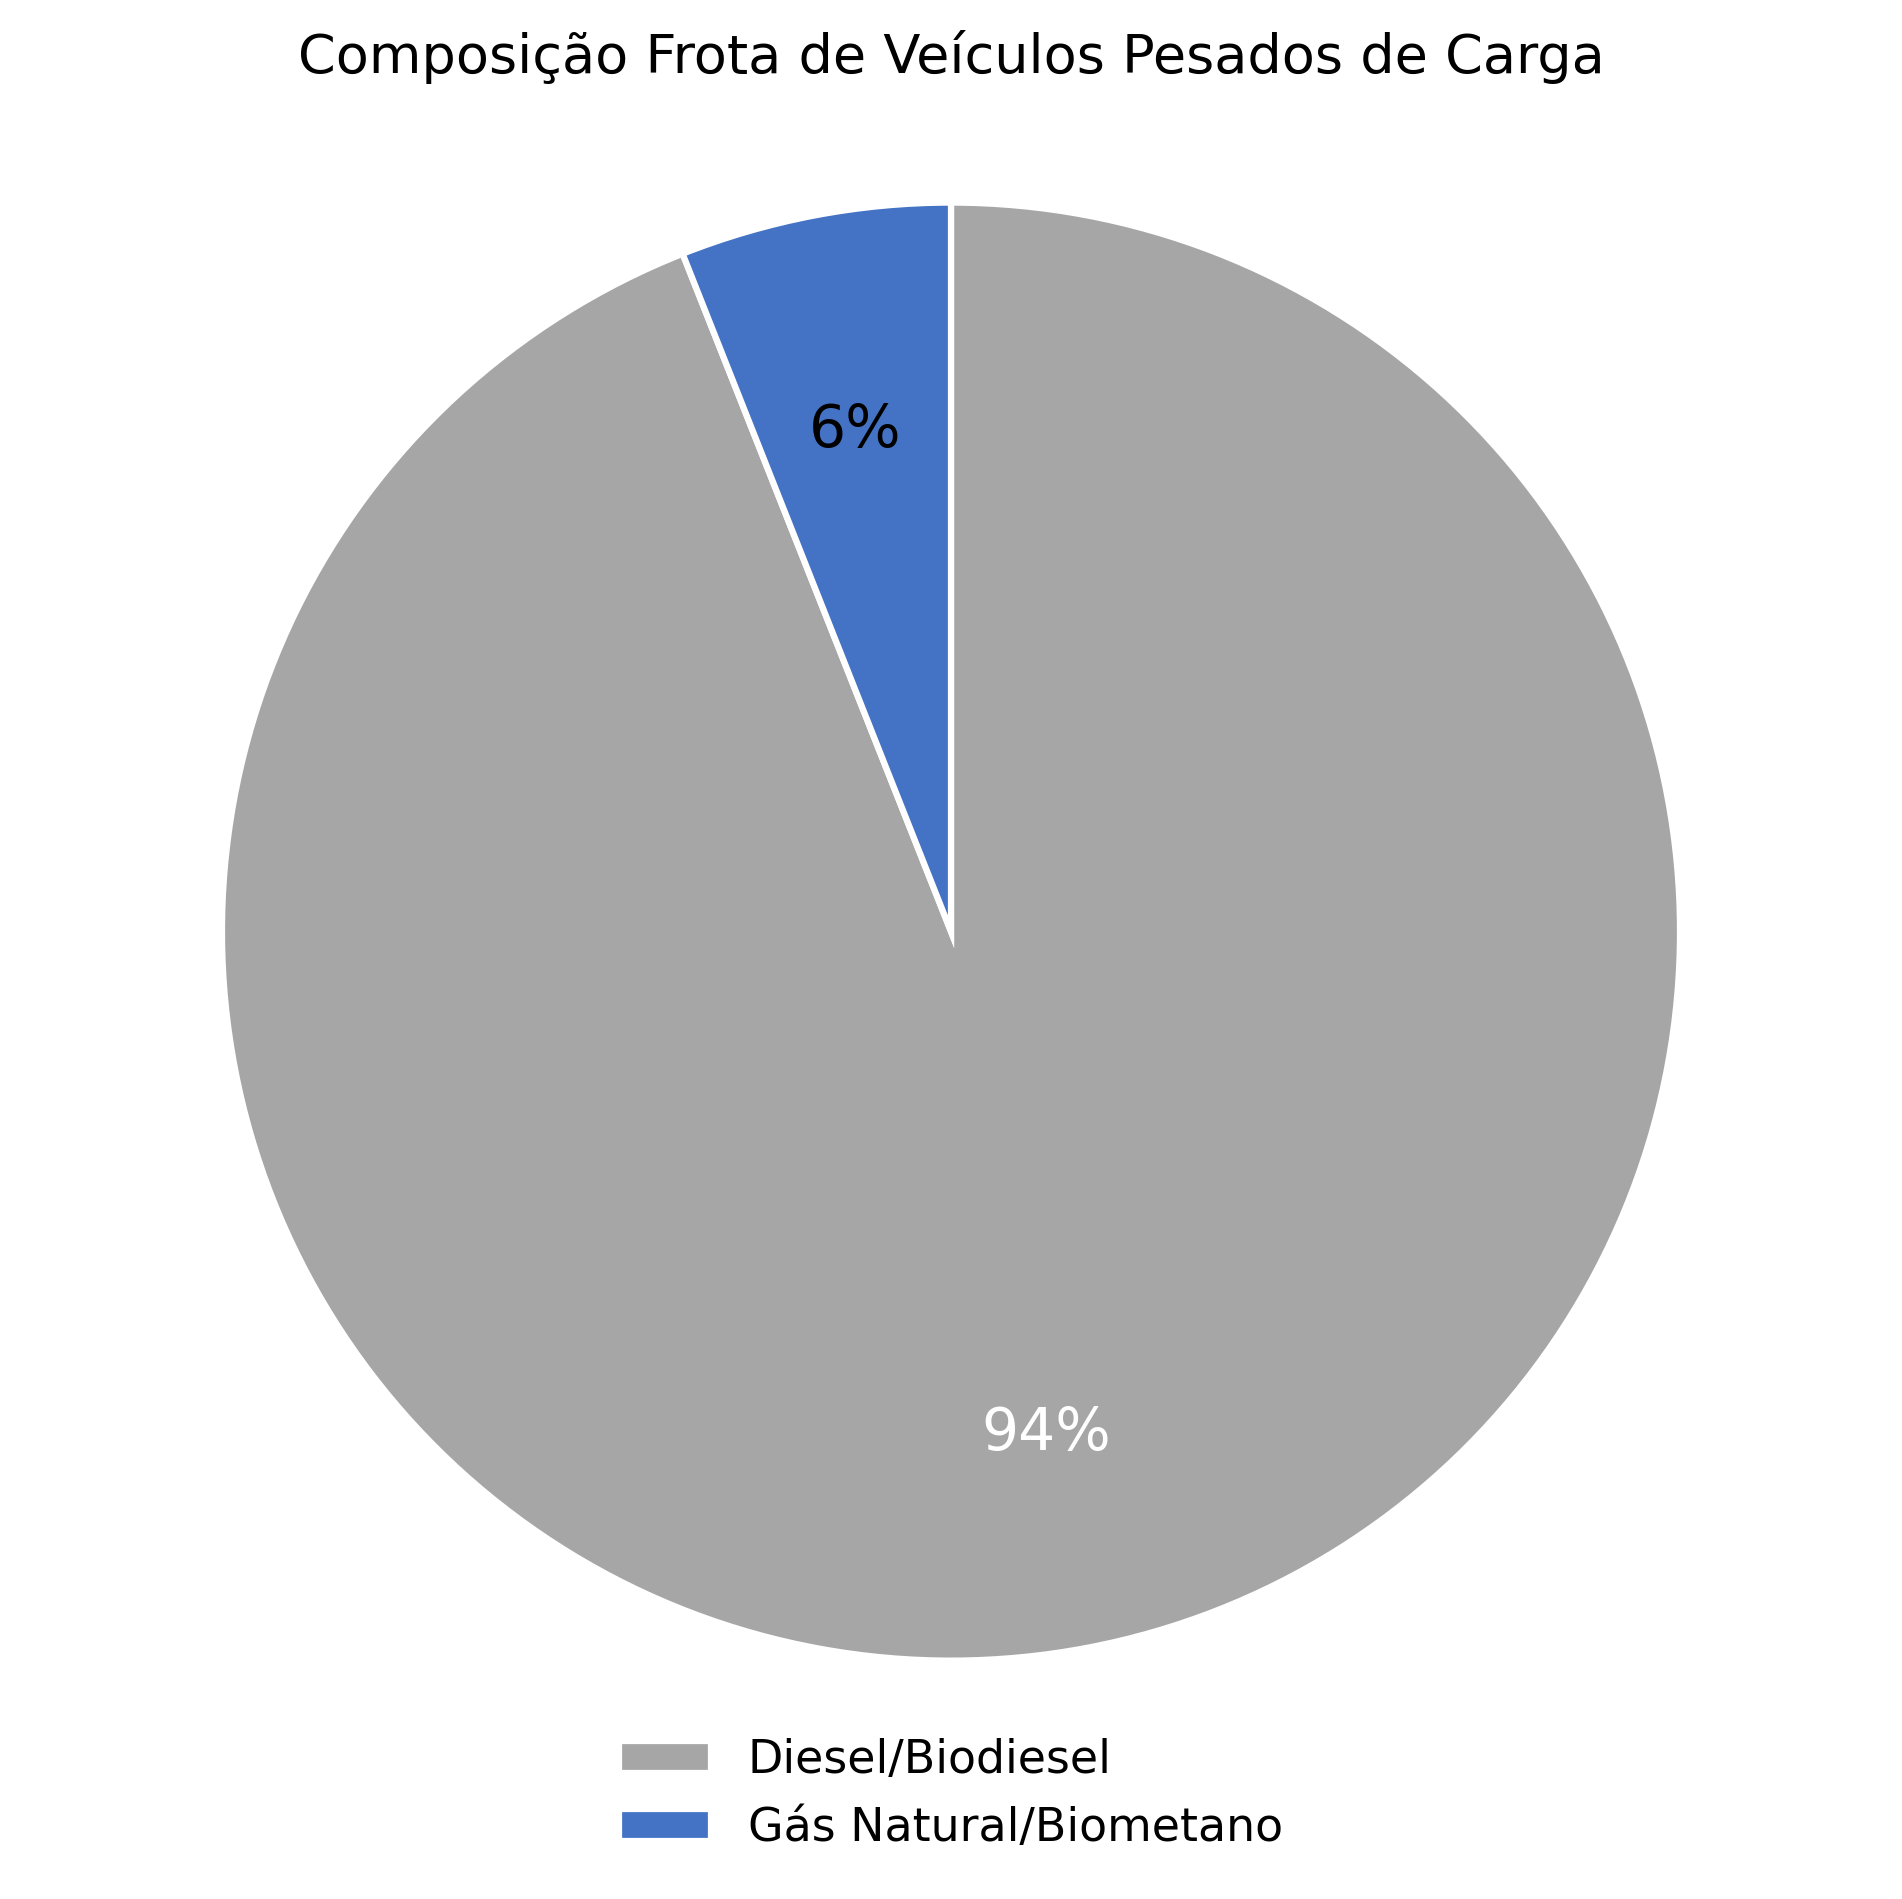
\includegraphics[width=0.55\textwidth]{figuras/frota_pesados_carga.png}
    \caption{Composição dos veículos pesados de carga por energético
             (diesel/biodiesel e gás natural/biometano).}
    \label{fig:frota-pesados}
    \fonte{elaborada com base em \citeonline{EPE2025}.}
\end{figure}

Diante da projeção de que apenas uma fração marginal ($\sim$2\%) da frota de
caminhões será composta por veículos elétricos \pendente{indicar a fonte do valor
de 2\%}, e da ausência de séries comparáveis às dos veículos leves para os ônibus,
os veículos pesados não integram os cenários quantitativos deste trabalho
(Seção~\ref{sec:met-cenarios}).

\subsubsection{Cenários Adotados}
\label{subsec:cenarios-sensibilidade}

Conforme a Seção~\ref{sec:met-cenarios}, os cenários \textbf{Conservador} e
\textbf{Acelerado} correspondem, respectivamente, aos cenários de transição
gradual e acelerada do estudo ANFAVEA/BCG. A
Tabela~\ref{tab:cenarios-adotados} resume as faixas resultantes para a frota
eletrificada de veículos leves.

\begin{table}[H]
\centering
\caption{Cenários de eletrificação da frota de veículos leves adotados neste
         trabalho (milhões de veículos).}
\label{tab:cenarios-adotados}
\small
\begin{tabular}{lcccccc}
\toprule
 & \multicolumn{2}{c}{\textbf{2030}} & \multicolumn{2}{c}{\textbf{2035}} &
   \multicolumn{2}{c}{\textbf{2040}} \\
\cmidrule(lr){2-3}\cmidrule(lr){4-5}\cmidrule(lr){6-7}
\textbf{Agregado} & \textbf{Cons.} & \textbf{Acel.} & \textbf{Cons.} &
\textbf{Acel.} & \textbf{Cons.} & \textbf{Acel.} \\
\midrule
Eletrificados, incluindo MHEV & 5 & 6 & 12 & 14 & 26 & 28 \\
Eletrificados, sem MHEV       & 3 & 4 &  8 & 10 & 18 & 22 \\
BEV + PHEV                    & 2 & 3 &  5 &  6 & 11 & 14 \\
\bottomrule
\end{tabular}
\fonte{elaborada com base na Tabela~\ref{tab:bcg} \cite{anfaveabcg2024}.}
\end{table}

Os dois cenários delimitam uma frota eletrificada de 5 a 6~milhões de veículos em
2030, de 12 a 14~milhões em 2035 e de 26 a 28~milhões em 2040, incluídos os
híbridos leves (MHEV); sem eles, de 3 a 4, de 8 a 10 e de 18 a 22~milhões. Para a
massa de baterias, os segmentos determinantes são o BEV e o PHEV
(Tabela~\ref{tab:categoria-massa}), que passam de 2--3~milhões em 2030 para
11--14~milhões em 2040.

A verificação cruzada com as demais fontes
(Figuras~\ref{fig:comparacao-frotas} e~\ref{fig:composicao-frota}) indica que:
(i)~a projeção da Bright Consulting para 2030 (6,5--7~milhões) situa-se acima de
ambos os cenários, mesmo com os MHEV; (ii)~a do PDE~2035 (3,7~milhões em 2035)
situa-se muito abaixo da faixa sem MHEV (8--10~milhões), refletindo a premissa de
renovação lenta da frota; e (iii)~a do MBC Brasil para 2040 (17,4~milhões) é
próxima do cenário Conservador sem MHEV (18~milhões). A faixa adotada é, portanto,
intermediária entre as projeções disponíveis, o que reforça seu uso como envelope
para análises futuras de demanda de materiais, mas depende da composição de cada
fonte, que nem sempre explicita a inclusão dos MHEV.

% ===========================================================
\subsection{Da Frota à Fábrica}
\label{sec:frota-fabrica}
% ===========================================================

Os resultados deste capítulo motivam o estudo industrial do
Capítulo~\ref{sec:gigafabrica} por três razões. Primeiro, o LFP é a química mais
frequente na amostra analisada (48,12\%) e predomina entre os BEV — nove dos doze
modelos da Tabela~\ref{tab:bev} —, categoria que concentra a maior parte da massa
de baterias (Tabela~\ref{tab:categoria-massa}). Segundo, ambos os cenários
projetam crescimento expressivo de BEV e PHEV, de 2--3~milhões em 2030 para
11--14~milhões de veículos em 2040 (Tabela~\ref{tab:cenarios-adotados}), o que
torna relevante compreender os fluxos de materiais e de energia da produção das
células que os equiparão. Terceiro, a fabricação de células gera, desde o início
da operação, um fluxo de material secundário homogêneo — a sucata de produção —,
que antecede os volumes de baterias pós-consumo e pode sustentar as primeiras
etapas de uma cadeia nacional de reciclagem
(Seção~\ref{subsec:sintese-reciclagem}).

O estudo industrial não modela a frota nem um conjunto de fábricas: quantifica os
fluxos por kWh de célula LFP e os normaliza para 1~GWh de produção anual. A
conversão dos cenários de frota em demanda anual de células, em GWh/ano, exigiria
capacidades médias de bateria por categoria e taxas de reposição, não levantadas
nesta etapa, e integra a continuidade do trabalho.

\newpage
\section{Análise de Fluxo de Materiais e Energia de uma Fábrica}
\label{sec:gigafabrica}

Este capítulo apresenta uma Análise de Fluxo de Materiais e Energia (MEFA) para
uma fábrica de células de bateria do tipo LFP (LiFePO\textsubscript{4}),
complementando a análise em escala de frota com uma visão em escala de processo
industrial. Os valores apresentados correspondem a faixas de referência
consolidadas na literatura técnica sobre manufatura de células
\citep{knehr2022batpac,degen2022,erakca2021,dai2019}, e não a medições de uma
planta específica. Sendo assim, os valores devem ser interpretados como ordens de grandeza
representativas e aproximadas.

% ===========================================================
\subsection{Bases de Cálculo e Fronteiras do Sistema}
\label{subsec:giga-bases}
% ===========================================================

A análise adota como unidade \textbf{1~kWh de célula LFP acabada e
testada}, escalonada para uma capacidade produtiva de \textbf{1~GWh/ano}. Os
parâmetros de referência estão reunidos na Tabela~\ref{tab:giga-bases}.

\begin{table}[H]
\centering
\caption{Parâmetros de referência da análise.}
\label{tab:giga-bases}
\small
\renewcommand{\arraystretch}{1.2}
\begin{tabularx}{\textwidth}{@{} >{\raggedright\arraybackslash}p{5.2cm} >{\raggedright\arraybackslash}p{3.4cm} X @{}}
\toprule
\textbf{Parâmetro} & \textbf{Valor adotado} & \textbf{Observação} \\
\midrule
Unidade funcional & 1~kWh de célula & Escalonado para 1~GWh/ano ($\times 10^{6}$) \\
Formato de referência & Prismática, invólucro de Al & Formato dominante em LFP automotivo \\
Densidade energética da célula & 160~Wh/kg & Faixa atual: 150--180~Wh/kg \\
Massa de célula & 6,25~kg/kWh & $1000~\text{Wh} \div 160~\text{Wh/kg}$ \\
Tensão nominal & 3,2~V & Característica do LiFePO\textsubscript{4} \\
Produção anual & 1~GWh/ano & $\approx$~6.250~t de células/ano \\
Taxa de refugo global & 8\% &  \textit - \\
\bottomrule
\end{tabularx}
\fonte{elaborada pelos autores com base em \citet{knehr2022batpac}.}
\end{table}

A fronteira do sistema é do tipo \textit{gate-to-gate}: compreende exclusivamente
as operações entre o recebimento das matérias-primas no portão da fábrica e a
expedição da célula acabada. Estão \textbf{incluídos} no escopo todas as etapas
de fabricação da célula (mistura, revestimento, secagem, calandragem, corte,
montagem, enchimento, formação, envelhecimento e teste), os circuitos internos
de recuperação (NMP, água e sucata metálica), as utilidades consumidas na planta
e as emissões no ponto de descarga. Estão \textbf{excluídos} a mineração e o
refino dos minerais, a síntese do material ativo de catodo (tratado como insumo
adquirido), a montagem de módulos e \textit{packs}, as fases de uso e fim de
vida, o transporte e a construção da planta. Para plantas verticalmente
integradas, que sintetizam o LiFePO\textsubscript{4} a partir de
FePO\textsubscript{4} e Li\textsubscript{2}CO\textsubscript{3}, a fronteira deve
ser expandida; a Tabela~\ref{tab:giga-catodo} apresenta ambas as visões.

% ===========================================================
\subsection{Matriz Geral de Fluxos}
\label{subsec:giga-matriz}
% ===========================================================

\subsubsection{Entradas de Materiais}

As Tabelas~\ref{tab:giga-catodo} a~\ref{tab:giga-estrutural} detalham as
entradas de materiais por componente da célula.

\begin{table}[H]
\centering
\caption{Entradas do catodo por kWh e por GWh.}
\label{tab:giga-catodo}
\small
\renewcommand{\arraystretch}{1.15}
\begin{tabularx}{\textwidth}{@{} >{\raggedright\arraybackslash}p{5.4cm} r r X @{}}
\toprule
\textbf{Item} & \textbf{kg/kWh} & \textbf{t/GWh} & \textbf{Observação} \\
\midrule
\textbf{LiFePO\textsubscript{4}} & 2,15 & 2.150 & $\sim$34\% da massa da célula \\
\multicolumn{4}{@{}l}{\textit{Alternativa --- planta integrada:}} \\
\quad FePO\textsubscript{4} (precursor) & 2,10 & 2.100 & 0,956~kg/kg (estequiometria) \\
\quad Li\textsubscript{2}CO\textsubscript{3} (grau bateria) & 0,55 & 550 & 0,53~kg LCE teórico + perdas \\
\quad Fonte de carbono (sacarose/glicose) & 0,10 & 100 & Precursor do revestimento de C \\
Negro de fumo & 0,07 & 70 & Aditivo condutor \\
PVDF (aglutinante) & 0,08 & 80 & Dissolvido em NMP \\
\midrule
\textbf{Subtotal do revestimento catódico} & \textbf{2,30} & \textbf{2.300} & Base seca \\
\bottomrule
\end{tabularx}
\fonte{elaborada pelos autores com base em \citet{knehr2022batpac} e \citet{dai2019}.}
\end{table}

O conteúdo de lítio da célula pode ser verificado por estequiometria. O
LiFePO\textsubscript{4} ($M = 157{,}76$~g/mol) contém 4,40\% de lítio em massa,
e o LiPF\textsubscript{6} ($M = 151{,}9$~g/mol), 4,57\%:
\begin{equation}
m_{\text{Li}} = \underbrace{2{,}15 \times 0{,}0440}_{\text{catodo}}
              + \underbrace{0{,}11 \times 0{,}0457}_{\text{eletrólito}}
              \approx 0{,}100~\text{kg Li/kWh}
\label{eq:giga-litio}
\end{equation}
o que equivale a aproximadamente \textbf{0,53~kg de carbonato de lítio
equivalente (LCE) por kWh}, ou 532~t~LCE por GWh --- valor consistente com a
faixa de 0,5--0,6~kg~LCE/kWh usualmente adotada para a química LFP.

\begin{table}[H]
\centering
\caption{Entradas do anodo por kWh e por GWh.}
\label{tab:giga-anodo}
\small
\renewcommand{\arraystretch}{1.15}
\begin{tabularx}{\textwidth}{@{} >{\raggedright\arraybackslash}p{5.4cm} r r X @{}}
\toprule
\textbf{Item} & \textbf{kg/kWh} & \textbf{t/GWh} & \textbf{Observação} \\
\midrule
Grafite (sintético ou natural) & 1,18 & 1.180 & $\sim$94\% do revestimento anódico \\
Negro de fumo & 0,03 & 30 & Aditivo condutor \\
CMC (carboximetilcelulose) & 0,015 & 15 & Espessante, sistema aquoso \\
SBR (estireno-butadieno) & 0,025 & 25 & Aglutinante elastomérico \\
\midrule
\textbf{Subtotal do revestimento anódico} & \textbf{1,25} & \textbf{1.250} & Base seca \\
\bottomrule
\end{tabularx}
\fonte{elaborada pelos autores com base em \citet{knehr2022batpac}.}
\end{table}

\begin{table}[H]
\centering
\caption{Solventes, eletrólito e separador.}
\label{tab:giga-solventes}
\small
\renewcommand{\arraystretch}{1.15}
\begin{tabularx}{\textwidth}{@{} >{\raggedright\arraybackslash}p{5.4cm} r r X @{}}
\toprule
\textbf{Item} & \textbf{kg/kWh} & \textbf{t/GWh} & \textbf{Observação} \\
\midrule
NMP --- circulante bruto & 1,60 & 1.600 & Pasta catódica a $\sim$60\% de sólidos \\
NMP --- reposição líquida & 0,012 & 12 & Após recuperação de 99,3\% \\
Água deionizada (pasta anódica) & 1,30 & 1.300 & Pasta aquosa a $\sim$50\% de sólidos \\
\textbf{Eletrólito total} & \textbf{0,85} & \textbf{850} & $\sim$13,5\% da massa da célula \\
\quad LiPF\textsubscript{6} (sal) & 0,11 & 110 & $\sim$13\% do eletrólito \\
\quad Carbonatos (EC/DMC/EMC) & 0,72 & 720 & Solventes orgânicos \\
\quad Aditivos (VC, FEC) & 0,02 & 20 & Formadores de SEI \\
Separador (PP/PE) & 0,14 & 140 & 12--20~\textmu m \\
\bottomrule
\end{tabularx}
\fonte{elaborada pelos autores com base em \citet{knehr2022batpac} e \citet{degen2022}.}
\end{table}

\begin{table}[H]
\centering
\caption{Componentes estruturais.}
\label{tab:giga-estrutural}
\small
\renewcommand{\arraystretch}{1.15}
\begin{tabularx}{\textwidth}{@{} >{\raggedright\arraybackslash}p{5.4cm} r r X @{}}
\toprule
\textbf{Item} & \textbf{kg/kWh} & \textbf{t/GWh} & \textbf{Observação} \\
\midrule
Folha de cobre (coletor anódico) & 0,62 & 620 & 6--8~\textmu m \\
Folha de alumínio (coletor catódico) & 0,26 & 260 & 12--15~\textmu m \\
Invólucro, tampa, terminais e \textit{vent} (Al) & 0,80 & 800 & Célula prismática \\
Fitas isolantes e diversos & 0,08 & 80 & --- \\
\midrule
\textbf{Subtotal estrutural} & \textbf{1,76} & \textbf{1.760} & $\sim$28\% da massa da célula \\
\bottomrule
\end{tabularx}
\fonte{elaborada pelos autores com base em \citet{knehr2022batpac}.}
\end{table}

A Tabela~\ref{tab:giga-balanco-celula} consolida o balanço de massa da célula
acabada.

\begin{table}[H]
\centering
\caption{Balanço de massa da célula LFP acabada.}
\label{tab:giga-balanco-celula}
\small
\renewcommand{\arraystretch}{1.15}
\begin{tabular}{@{} l r r @{}}
\toprule
\textbf{Componente} & \textbf{kg/kWh} & \textbf{\% da massa} \\
\midrule
Revestimento catódico & 2,30 & 36,8 \\
Revestimento anódico & 1,25 & 20,0 \\
Eletrólito & 0,85 & 13,6 \\
Invólucro e terminais & 0,80 & 12,8 \\
Folha de Cu & 0,62 & 9,9 \\
Folha de Al & 0,26 & 4,2 \\
Separador & 0,14 & 2,2 \\
Diversos & 0,08 & 1,3 \\
\midrule
\textbf{Total} & \textbf{6,30} & \textbf{100,0} \\
\bottomrule
\end{tabular}
\fonte{elaborada pelos autores.}
\end{table}

A soma de componentes (6,30~kg/kWh) difere ligeiramente da massa nominal
(6,25~kg/kWh) em função de arredondamentos. Considerando a taxa de refugo global
de 8\%, o consumo efetivo de matéria-prima eleva-se a aproximadamente
\textbf{6,79~kg/kWh} ($6{,}25 \div 0{,}92$), dos quais cerca de 0,54~kg/kWh
retornam como sucata, parcialmente recuperável.

\subsubsection{Utilidades}

\begin{table}[H]
\centering
\caption{Consumo de utilidades por kWh de célula produzida.}
\label{tab:giga-utilidades}
\small
\renewcommand{\arraystretch}{1.15}
\begin{tabularx}{\textwidth}{@{} >{\raggedright\arraybackslash}p{4.8cm} r l X @{}}
\toprule
\textbf{Utilidade} & \textbf{Valor} & \textbf{Unidade} & \textbf{Faixa da literatura} \\
\midrule
Energia elétrica & 35 & kWh/kWh & 30--50 (madura); 55--80 (\textit{ramp-up}) \\
Energia térmica (gás natural) & 3--8 & kWh/kWh & Plantas não eletrificadas \\
Água industrial (captação) & 25--60 & L/kWh & Depende do resfriamento \\
Água deionizada & 1,3--2,0 & L/kWh & Pasta anódica e limpeza \\
Nitrogênio (N\textsubscript{2}) & 1,5--3,0 & Nm\textsuperscript{3}/kWh & Inertização e enchimento \\
Argônio (Ar) & 0,05--0,2 & Nm\textsuperscript{3}/kWh & Soldagem a laser \\
Ar comprimido & 3--8 & Nm\textsuperscript{3}/kWh & Pneumática geral \\
\bottomrule
\end{tabularx}
\fonte{elaborada pelos autores com base em \citet{degen2022} e \citet{erakca2021}.}
\end{table}

\subsubsection{Circuitos Internos de Recuperação}

A Tabela~\ref{tab:giga-loops} apresenta os circuitos internos que recirculam
massa e energia sem que estas cruzem a fronteira do sistema.

\begin{table}[H]
\centering
\caption{Circuitos internos de recuperação e reutilização.}
\label{tab:giga-loops}
\small
\renewcommand{\arraystretch}{1.2}
\begin{tabularx}{\textwidth}{@{} >{\raggedright\arraybackslash}p{3.4cm} >{\raggedright\arraybackslash}p{2.2cm} >{\raggedright\arraybackslash}p{2.6cm} X @{}}
\toprule
\textbf{Circuito} & \textbf{Recuperação} & \textbf{Fluxo recirculado} & \textbf{Descrição} \\
\midrule
Recuperação de NMP & 99,0--99,5\% & 1,59~kg/kWh & Condensação do vapor da secagem, destilação a vácuo e desidratação; retorna à mistura com pureza $>$99,5\% \\
\addlinespace
Sucata de eletrodo (pasta) & 60--80\% & 0,20--0,30~kg/kWh & Pasta fora de especificação retorna à mistura sem reprocessamento químico \\
\addlinespace
Sucata de eletrodo (revestido) & Externa & 0,15--0,25~kg/kWh & Delaminação; \textit{black mass} enviada a reciclador e folhas vendidas como sucata \\
\addlinespace
Aparas metálicas & $>$95\% & 0,05--0,09~kg/kWh & Cu e Al limpos do corte de borda \\
\addlinespace
Água de resfriamento & 92--97\% & 20--50~L/kWh & Torres com purga controlada \\
\addlinespace
Condensado da sala seca & 70--85\% & 2--5~L/kWh & Água da desumidificação retorna às utilidades \\
\addlinespace
Energia da formação & 30--50\% & 1--3~kWh/kWh & Descarga realimentada à rede interna por conversores bidirecionais \\
\bottomrule
\end{tabularx}
\fonte{elaborada pelos autores com base em \citet{degen2022} e \citet{knehr2022batpac}.}
\end{table}

A recuperação de NMP é imprescindível por duas razões: o solvente é
classificado como substância de elevada preocupação (SVHC) no regulamento
europeu REACH, por toxicidade reprodutiva, e seu custo de reposição
inviabilizaria a operação. Taxas inferiores a 98\%
comprometem simultaneamente a conformidade ambiental e a viabilidade econômica
da planta.

\subsubsection{Saídas: Produto, Subprodutos e Emissões}

\begin{table}[H]
\centering
\caption{Saídas de produto e subprodutos.}
\label{tab:giga-saidas}
\small
\renewcommand{\arraystretch}{1.15}
\begin{tabularx}{\textwidth}{@{} >{\raggedright\arraybackslash}p{5.0cm} r r X @{}}
\toprule
\textbf{Fluxo} & \textbf{kg/kWh} & \textbf{t/GWh} & \textbf{Destino} \\
\midrule
\textbf{Células LFP aprovadas} & \textbf{6,25} & \textbf{6.250} & Produto principal \\
Células reprovadas no teste & 0,30--0,50 & 300--500 & Reciclagem externa \\
Sucata de Cu (limpa) & 0,05 & 50 & Venda como sucata \\
Sucata de Al (limpa) & 0,04 & 40 & Venda como sucata \\
\textit{Black mass} de produção & 0,15--0,25 & 150--250 & Reciclador externo \\
Pasta rejeitada & 0,05--0,10 & 50--100 & Resíduo classe I ou recuperação \\
\bottomrule
\end{tabularx}
\fonte{elaborada pelos autores.}
\end{table}

Cabe destacar que a sucata de produção é economicamente mais atrativa do que a
reciclagem pós-consumo de baterias LFP discutida na
Seção~\ref{subsec:lfp-economics}: a \textit{black mass} de fábrica é homogênea,
de composição conhecida e livre de contaminação, condição que viabiliza a
reciclagem direta --- rota inviável para a maior parte dos lotes pós-consumo.

\begin{table}[H]
\centering
\caption{Emissões e efluentes por kWh de célula produzida.}
\label{tab:giga-emissoes}
\small
\renewcommand{\arraystretch}{1.15}
\begin{tabularx}{\textwidth}{@{} >{\raggedright\arraybackslash}p{4.6cm} r l X @{}}
\toprule
\textbf{Fluxo} & \textbf{Valor} & \textbf{Unidade} & \textbf{Tratamento} \\
\midrule
VOCs (NMP e carbonatos) & 10--25 & g/kWh & Oxidação térmica regenerativa ou carvão ativado \\
Emissões fugitivas de eletrólito & 2--8 & g/kWh & Captação localizada \\
Gases de formação (CO\textsubscript{2}, CO, C\textsubscript{2}H\textsubscript{4}, H\textsubscript{2}) & 5--20 & g/kWh & Degasagem pós-formação \\
Material particulado & 0,5--2 & g/kWh & Filtros HEPA \\
Efluente líquido tratado & 15--40 & L/kWh & Estação de tratamento própria \\
Calor dissipado & 25--40 & \% da energia & HVAC e torres de resfriamento \\
\bottomrule
\end{tabularx}
\fonte{elaborada pelos autores com base em \citet{degen2022}.}
\end{table}

As emissões de escopo~2 dependem fortemente da matriz elétrica. Adotando fatores
de emissão aproximados de 0,10~kg\,CO\textsubscript{2}e/kWh para o Brasil e
0,58~kg\,CO\textsubscript{2}e/kWh para a China, o consumo de 35~kWh/kWh resulta
em cerca de \textbf{3,5~kg\,CO\textsubscript{2}e/kWh} no cenário brasileiro e
\textbf{20,3~kg\,CO\textsubscript{2}e/kWh} no chinês --- um diferencial de
aproximadamente seis vezes, o que favorece o argumento de produção nacional das células.

% ===========================================================
\subsection{Balanço por Etapa do Processo}
\label{subsec:giga-etapas}
% ===========================================================

\subsubsection{Mistura e Preparação das Pastas}

As pastas catódica e anódica são preparadas em misturadores ou
extrusoras de dupla rosca. A pasta catódica emprega NMP como solvente, com teor
de sólidos de 55--65\%, enquanto a anódica utiliza água deionizada, com 45--55\%
de sólidos. Por kWh, entram 2,30~kg de sólidos catódicos e 1,60~kg de NMP
(3,90~kg de pasta), além de 1,25~kg de sólidos anódicos e 1,30~kg de água
(2,55~kg de pasta). As perdas situam-se entre 1\% e 3\%, e o consumo energético,
entre 1,3 e 2,5~kWh/kWh. O teor de umidade do NMP deve ser mantido abaixo de
200~ppm, pois a água residual hidrolisa posteriormente o LiPF\textsubscript{6},
gerando ácido fluorídrico (HF).

\subsubsection{Revestimento, Secagem e Calandragem}

O revestimento é realizado por \textit{slot-die} a 50--80~m/min, seguido de
secagem em forno multizona a 80--160\,°C e calandragem até porosidade de
30--40\%. É nesta etapa que se evapora todo o solvente: 1,60~kg/kWh de NMP, dos
quais 1,59~kg são recuperados. Trata-se da etapa mais intensiva em energia de
toda a planta, conforme a Tabela~\ref{tab:giga-energia-coating}.

\begin{table}[H]
\centering
\caption{Consumo energético da etapa de revestimento e secagem.}
\label{tab:giga-energia-coating}
\small
\renewcommand{\arraystretch}{1.15}
\begin{tabular}{@{} l r r @{}}
\toprule
\textbf{Subsistema} & \textbf{kWh/kWh} & \textbf{\% da planta} \\
\midrule
Fornos de secagem & 8--12 & 25--30 \\
Recuperação e destilação de NMP & 4--7 & 12--18 \\
Exaustão e tratamento de ar & 1--2 & 3--5 \\
Calandragem & 0,3--0,6 & $\sim$1 \\
\midrule
\textbf{Subtotal} & \textbf{13--22} & \textbf{$\approx$45} \\
\bottomrule
\end{tabular}
\fonte{elaborada pelos autores com base em \citet{degen2022}.}
\end{table}

O revestimento a seco (\textit{dry coating}), ao eliminar o solvente, suprime
integralmente o forno de secagem e o circuito de NMP, com potencial de redução de
30--45\% no consumo energético da planta. A tecnologia encontra-se em TRL~6--7.

\subsubsection{Corte e Montagem}

Os eletrodos são cortados por lâmina rotativa ou laser e montados por
empilhamento (\textit{stacking}) em sala seca com ponto de orvalho de
$-40$\,°C. As aparas de corte representam 2--5\% da área revestida: 0,10 a
0,18~kg/kWh de eletrodo revestido, destinados à delaminação, e 0,05 a
0,09~kg/kWh de folha metálica limpa. O consumo energético, de 1,5 a
3,0~kWh/kWh, decorre majoritariamente da desumidificação da sala, e não do
processo mecânico.

\subsubsection{Injeção de Eletrólito e Selagem}

O eletrólito (2,0--2,6~g/Ah, ou $\approx$0,85~kg/kWh) é injetado a vácuo em
atmosfera de nitrogênio com ponto de orvalho de $-45$\,°C, seguido de
impregnação de 6 a 24~h e selagem por soldagem a laser. As perdas por
evaporação são de 2 a 8~g/kWh. O controle de umidade nesta etapa é
necessário para segurança, e não apenas qualidade, dado o risco de formação de HF
pela hidrólise do LiPF\textsubscript{6}.

\subsubsection{Formação, Degasagem e Envelhecimento}

A formação consiste em 2 a 5 ciclos parciais de carga a C/20--C/10, com duração
de 12 a 36~h, durante os quais se constitui a interface sólido-eletrólito (SEI)
e se liberam de 5 a 20~g/kWh de gases. Segue-se o envelhecimento de 7 a 21~dias
a 25--45\,°C, com taxa de reprovação de 3--8\%. O consumo energético líquido é de
4 a 7~kWh/kWh, dos quais 1 a 3~kWh/kWh são recuperados na descarga. Mais do que
energético, este é o principal gargalo de capital da planta: o tempo de
residência de até três semanas exige grandes áreas de armazenamento climatizado.

% ===========================================================
\subsection{Indicadores de Eficiência}
\label{subsec:giga-indicadores}
% ===========================================================

\begin{table}[H]
\centering
\caption{Rendimento de massa e taxas de refugo por etapa.}
\label{tab:giga-rendimento}
\small
\renewcommand{\arraystretch}{1.15}
\begin{tabular}{@{} l c c c @{}}
\toprule
\textbf{Indicador} & \textbf{Planta Consolidada} & \textbf{\textit{Ramp-up}} & \textbf{Melhor prática} \\
\midrule
Rendimento global de massa & 92\% & 70--85\% & 95--96\% \\
Taxa de refugo global & 8\% & 15--30\% & 4--5\% \\
\quad Mistura & 1--3\% & 5--8\% & $<$1\% \\
\quad Revestimento e secagem & 2--4\% & 8--15\% & 1,5\% \\
\quad Corte e montagem & 2--5\% & 5--10\% & 1,5\% \\
\quad Formação e teste & 3--8\% & 10--20\% & 1--2\% \\
Fração do refugo recuperada & 75--85\% & 60--70\% & $>$90\% \\
\bottomrule
\end{tabular}
\fonte{elaborada pelos autores com base em \citet{degen2022}.}
\end{table}

O rendimento efetivo de material, considerando a recuperação de 80\% da sucata
gerada, é dado por:
\begin{equation}
\eta_{\text{efetivo}} = \frac{m_{\text{célula}} + m_{\text{recuperado}}}{m_{\text{entrada}}}
= \frac{6{,}25 + 0{,}43}{6{,}79} \approx 98{,}4\%
\label{eq:giga-rendimento}
\end{equation}

A recuperação de NMP, de 99,0 a 99,5\%, limita a reposição a 8--16~g/kWh
(8--16~t/GWh por ano), com pureza do solvente recuperado superior a 99,5\% e
consumo energético de destilação de 4 a 7~kWh/kWh.

A intensidade energética é o parâmetro mais disperso da literatura, variando de
20 a mais de 100~kWh/kWh conforme a fronteira adotada e a escala da planta
\citep{degen2022,erakca2021}. A Tabela~\ref{tab:giga-intensidade} sintetiza os
cenários e a Figura~\ref{fig:giga-energia} apresenta a distribuição do consumo
no cenário de referência.

\begin{table}[H]
\centering
\caption{Intensidade energética por cenário de maturidade.}
\label{tab:giga-intensidade}
\small
\renewcommand{\arraystretch}{1.15}
\begin{tabularx}{\textwidth}{@{} >{\raggedright\arraybackslash}p{5.6cm} c X @{}}
\toprule
\textbf{Cenário} & \textbf{kWh/kWh} & \textbf{Observação} \\
\midrule
\textit{Ramp-up} ou planta pequena ($<$2~GWh) & 55--80 & Baixa utilização da capacidade \\
\textbf{Planta madura (referência)} & \textbf{30--50} & Valor central adotado: 35 \\
Melhor prática ($>$20~GWh) & 25--32 & Economia de escala em utilidades \\
Com revestimento a seco & 15--22 & Projeção; ainda não comercial \\
\bottomrule
\end{tabularx}
\fonte{elaborada pelos autores com base em \citet{degen2022}.}
\end{table}

\begin{figure}[H]
\centering
\begin{tikzpicture}
\begin{axis}[
    xbar,
    width  = 12cm,
    height = 6.2cm,
    bar width = 12pt,
    xmin = 0, xmax = 16,
    xlabel = {Consumo elétrico (kWh por kWh de célula)},
    xlabel style = {font=\footnotesize},
    symbolic y coords = {Utilidades gerais,Processos mecânicos,Formação e envelhecimento,Sala seca,Secagem e recuperação de NMP},
    ytick = data,
    yticklabel style = {font=\footnotesize},
    xticklabel style = {font=\footnotesize},
    nodes near coords,
    nodes near coords style = {font=\footnotesize},
    every node near coord/.append style = {/pgf/number format/use comma},
    xmajorgrids = true,
    grid style = {dotted, gray!40},
    axis x line* = bottom,
    axis y line* = left,
    enlarge y limits = 0.15,
]
\addplot[fill=gigaAzul, draw=none] coordinates {
    (3.5,Utilidades gerais)
    (3.5,Processos mecânicos)
    (5.5,Formação e envelhecimento)
    (9.5,Sala seca)
    (13.0,Secagem e recuperação de NMP)
};
\end{axis}
\end{tikzpicture}
\caption{Distribuição do consumo de energia elétrica no cenário de referência
         (total de 35~kWh/kWh).}
\label{fig:giga-energia}
\fonte{elaborada pelos autores com base em \citet{degen2022}.}
\end{figure}

Observa-se que 64\% do consumo elétrico concentra-se na secagem e na sala seca
--- etapas que não promovem qualquer transformação química do material, limitando-se
a remover solvente e controlar a umidade. Essa constatação explica por que o
revestimento a seco é considerado uma inovação, mas não um ganho para o setor.

Por fim, a Tabela~\ref{tab:giga-sintese} reúne os indicadores-síntese para a
capacidade de referência.

\begin{table}[H]
\centering
\caption{Indicadores-síntese para uma planta de 1~GWh/ano.}
\label{tab:giga-sintese}
\small
\renewcommand{\arraystretch}{1.15}
\begin{tabular}{@{} l r @{}}
\toprule
\textbf{Indicador} & \textbf{Valor anual} \\
\midrule
Massa de células produzidas & 6.250~t \\
Matéria-prima consumida & 6.790~t \\
Lítio contido (LCE) & 532~t \\
Grafite & 1.180~t \\
Cobre & 620~t \\
Alumínio (folha e invólucro) & 1.060~t \\
Consumo elétrico & 35~GWh \\
Captação de água & 25.000--60.000~m\textsuperscript{3} \\
Refugo não recuperado & 110~t \\
Emissão de VOCs & 10--25~t \\
CO\textsubscript{2}e escopo~2 --- matriz brasileira & $\sim$3.500~t \\
CO\textsubscript{2}e escopo~2 --- matriz chinesa & $\sim$20.300~t \\
\bottomrule
\end{tabular}
\fonte{Elaborado por este trabalho.}
\end{table}

% ===========================================================
\subsection{Representação do Sistema}
\label{subsec:giga-diagrama}
% ===========================================================

A Figura~\ref{fig:giga-fluxo} apresenta o diagrama de fluxo do sistema,
organizado em quatro colunas: entradas, etapas de processo, circuitos internos e
saídas.

\begin{figure}[H]
\centering
\resizebox{\textwidth}{!}{%
\begin{tikzpicture}[
    font=\scriptsize,
    base/.style    = {rectangle, rounded corners=2pt, draw, thick, align=center,
                      minimum height=0.95cm, text width=3.1cm},
    entrada/.style = {base, draw=gigaAzul, fill=gigaAzul!12, text width=3.3cm},
    proc/.style    = {base, draw=black!60, fill=gray!10, text width=4.5cm},
    loop/.style    = {base, draw=gigaLaranja, fill=gigaLaranja!12},
    saida/.style   = {base, draw=gigaVerde, fill=gigaVerde!12},
    util/.style    = {base, draw=gigaRoxo, fill=gigaRoxo!10, text width=8cm},
    fluxo/.style   = {-{Latex[length=2.2mm]}, thick},
    aux/.style     = {-{Latex[length=2mm]}, dashed, thick},
]

% ---------- Etapas de processo ----------
\node[proc] (P1) at (0,  0.0) {\textbf{1. Mistura}\\pastas catódica e anódica};
\node[proc] (P2) at (0, -1.7) {\textbf{2. Revestimento e secagem}\\80--160\,°C $\cdot$ 13--22 kWh/kWh};
\node[proc] (P3) at (0, -3.4) {\textbf{3. Calandragem}\\porosidade 30--40\%};
\node[proc] (P4) at (0, -5.1) {\textbf{4. Corte e montagem}\\sala seca a $-40$\,°C};
\node[proc] (P5) at (0, -6.8) {\textbf{5. Enchimento e selagem}\\injeção a vácuo};
\node[proc] (P6) at (0, -8.5) {\textbf{6. Formação e envelhecimento}\\4--7 kWh/kWh};
\node[proc] (P7) at (0,-10.2) {\textbf{7. Teste e classificação}};

% ---------- Utilidades ----------
\node[util] (U) at (0, 2.4) {\textbf{Utilidades:} eletricidade 35 kWh/kWh $\cdot$ N\textsubscript{2}/Ar $\cdot$ água 25--60 L/kWh};

% ---------- Entradas ----------
\node[entrada] (I1) at (-5.3, 0.55) {LiFePO\textsubscript{4}, PVDF e negro de fumo\\2,30 kg/kWh};
\node[entrada] (I2) at (-5.3,-0.55) {Grafite, CMC e SBR\\1,25 kg/kWh};
\node[entrada] (I3) at (-5.3,-1.75) {NMP 1,60 e água DI 1,30\\kg/kWh};
\node[entrada] (I4) at (-5.3,-2.95) {Folhas Cu 0,62 e Al 0,26\\kg/kWh};
\node[entrada] (I5) at (-5.3,-5.1)  {Separador PP/PE\\0,14 kg/kWh};
\node[entrada] (I6) at (-5.3,-6.3)  {Eletrólito (LiPF\textsubscript{6})\\0,85 kg/kWh};
\node[entrada] (I7) at (-5.3,-7.4)  {Invólucro de Al\\0,80 kg/kWh};

% ---------- Circuitos internos ----------
\node[loop] (L2) at (5.4,  0.8) {Pasta rejeitada\\retorno 0,20--0,30 kg/kWh};
\node[loop] (L1) at (5.4, -1.7) {Recuperação de NMP\\99,0--99,5\% (1,59 kg/kWh)};
\node[loop] (L3) at (5.4, -5.1) {Aparas de corte\\0,15--0,27 kg/kWh};
\node[loop] (L4) at (5.4, -9.3) {Energia da descarga\\1--3 kWh/kWh};

% ---------- Saídas ----------
\node[saida] (O4a) at (10.6, -1.7) {VOCs\\10--25 g/kWh};
\node[saida] (O5)  at (10.6, -3.0) {Efluente tratado\\15--40 L/kWh};
\node[saida] (O3)  at (10.6, -5.1) {Sucata Cu/Al e \textit{black mass}\\0,15--0,27 kg/kWh};
\node[saida] (O4b) at (10.6, -7.3) {Gases de formação e eletrólito fugitivo\\7--28 g/kWh};
\node[saida] (O6)  at (10.6, -9.3) {Calor dissipado\\25--40\% da energia};
\node[saida, very thick] (O1) at (10.6,-10.7) {\textbf{Células LFP}\\\textbf{6,25 kg/kWh}};
\node[saida] (O2)  at (10.6,-12.0) {Células reprovadas\\0,30--0,50 kg/kWh};

% ---------- Moldura do processo ----------
\begin{scope}[on background layer]
\node[draw=black!35, dashed, rounded corners, fill=gray!3, inner sep=6pt,
      fit=(P1)(P7), label={[font=\scriptsize\bfseries]below:Processo}] (PROC) {};
\end{scope}

% ---------- Fluxo principal de massa ----------
\foreach \a/\b in {P1/P2,P2/P3,P3/P4,P4/P5,P5/P6,P6/P7}
    \draw[fluxo] (\a) -- (\b);

\draw[fluxo] (I1.east) -- (P1.west |- I1.east);
\draw[fluxo] (I2.east) -- (P1.west |- I2.east);
\draw[fluxo] (I3.east) -- ++(0.55,0) |- (P1.west);
\draw[fluxo] (I4.east) -- ++(0.85,0) |- (P2.west);
\draw[fluxo] (I5.east) -- (P4.west);
\draw[fluxo] (I6.east) -- ++(0.55,0) |- (P5.west);
\draw[fluxo] (I7.east) -- ++(0.55,0) |- (P5.west);

\draw[fluxo] (P7.east) -- ++(1.2,0) |- (O1.west);
\draw[fluxo] (P7.east) -- ++(1.2,0) |- (O2.west);

% ---------- Utilidades ----------
\draw[aux, gigaRoxo] (U) -- (PROC.north);

% ---------- Circuitos internos ----------
% pasta rejeitada: sai da mistura e retorna a ela
\draw[aux, gigaLaranja] ([yshift=2.5mm]P1.east) -- ++(0.9,0) |- (L2.west);
\draw[aux, gigaLaranja] (L2.north) -- ++(0,0.3) -| ([xshift=8mm]P1.north);
% NMP: sai da secagem e retorna à mistura
\draw[aux, gigaLaranja] (P2.east) -- (L1.west);
\draw[aux, gigaLaranja] (L1.north) |- ([yshift=-2.5mm]P1.east);
% aparas de corte
\draw[aux, gigaLaranja] (P4.east) -- (L3.west);
% energia recuperada na formação
\draw[aux, gigaLaranja] ([yshift=-2mm]P6.east) -- ++(0.9,0) |- (L4.west);

% ---------- Saídas auxiliares ----------
\draw[aux, gigaVerde] (L1.east) -- (O4a.west);
\draw[aux, gigaVerde] ([yshift=-3.5mm]P2.east) -- ++(0.9,0) |- (O5.west);
\draw[aux, gigaVerde] (L3.east) -- (O3.west);
\draw[aux, gigaVerde] (P5.east) -- ++(5.6,0) |- (O4b.west);
\draw[aux, gigaVerde] ([yshift=2mm]P6.east) -- ++(6.0,0) |- (O4b.west);
\draw[aux, gigaVerde] (L4.east) -- (O6.west);

\end{tikzpicture}%
}
\caption{Diagrama de fluxo de materiais e energia da fábrica de células LFP
         (valores por kWh de célula). Setas contínuas: fluxo principal de massa;
         setas tracejadas: utilidades, circuitos internos e emissões.}
\label{fig:giga-fluxo}
\fonte{elaborada pelos autores.}
\end{figure}

A leitura do diagrama evidencia três aspectos centrais do sistema. Em primeiro
lugar, o NMP forma um circuito praticamente fechado: a entrada bruta de
1,60~kg/kWh é quase integralmente compensada pelo retorno de 1,59~kg/kWh, de
modo que a entrada efetiva pela fronteira do sistema corresponde apenas à
reposição de 8--16~g/kWh. Em segundo lugar, a energia não acompanha a massa:
os fluxos de utilidades concentram-se nas etapas de secagem e formação, que não
são as que movimentam a maior quantidade de material. Em terceiro lugar, o
destino da sucata depende da etapa em que é gerada: a pasta rejeitada na mistura
retorna ao processo sem perda de valor, enquanto o eletrodo já seco e calandrado
exige delaminação e deixa o sistema como \textit{black mass}. Cada ponto
percentual de refugo deslocado das etapas finais para a etapa de mistura
representa, portanto, ganho econômico direto.

% ===========================================================
\subsection{Limitações da Análise}
\label{subsec:giga-limitacoes}
% ===========================================================

A análise apresentada está sujeita a limitações que devem orientar sua
interpretação. Os valores correspondem a faixas consolidadas da literatura, e não
a medições de uma planta específica, variando conforme formato de célula, grau
de automação, escala e idade da linha. A intensidade energética, em particular,
apresenta grande dispersão entre estudos, sobretudo em razão de fronteiras de
sistema distintas. A densidade energética de 160~Wh/kg constitui uma escolha de
cenário, e todas as massas apresentadas escalam inversamente a esse valor.
Finalmente, por tratar-se de uma fronteira \textit{gate-to-gate}, a análise não
captura a pegada ambiental da produção das matérias-primas --- em especial do
material ativo de catodo, que em análises \textit{cradle-to-gate} responde por
parcela expressiva do impacto climático total da célula \citep{dai2019}.
\newpage
\section{Conclusão}
\label{sec:conclusao}

Este trabalho caracterizou a frota eletrificada brasileira quanto às químicas de
bateria e às trajetórias de eletrificação até 2040 e quantificou, por meio de uma
Análise de Fluxo de Materiais e Energia, os fluxos associados à fabricação de
células LFP. Os principais resultados, organizados por objetivo específico, são
os seguintes.

\paragraph{Linha de base das químicas (Objetivo~1).}
Na amostra de mais de 509~mil veículos eletrificados emplacados, predomina o LFP
(48,12\%), seguido do NMC (32,75\%) e do NiMH (18,38\%), em participações por
número de veículos. O LFP domina entre os BEV — nove dos doze modelos de maior
volume —, e o NiMH está associado aos híbridos convencionais da Toyota. Como a
massa de bateria por veículo varia em uma ordem de grandeza entre categorias, essa
linha de base precisa ser convertida em massa ou em capacidade antes de alimentar
uma análise de fluxo de materiais da frota: com o \textit{mix} de vendas do
PDE~2035, os BEV respondem por pouco mais de um quarto das vendas de eletrificados,
mas por cerca de três quartos da massa de baterias vendidas.

\paragraph{Cenários de eletrificação (Objetivo~2).}
Os cenários Conservador e Acelerado, construídos a partir do estudo ANFAVEA/BCG,
delimitam uma frota eletrificada de veículos leves de 5--6~milhões de veículos em
2030, 12--14~milhões em 2035 e 26--28~milhões em 2040, incluídos os híbridos leves;
os BEV e PHEV, que concentram a massa de baterias, passam de 2--3~milhões para
11--14~milhões. A faixa é intermediária entre as projeções disponíveis: a do
PDE~2035 é muito inferior, a da Bright Consulting para 2030 é superior, e a do MBC
Brasil para 2040 é próxima do cenário Conservador sem os híbridos leves.

\paragraph{Fluxos da fabricação de células LFP (Objetivo~3).}
No caso central, a fabricação de 1~kWh de célula LFP (6,25~kg) consome 6,66~kg de
materiais e gera 0,39~kg de refugo, com rendimento global de massa de 93,9\%; 97\%
do refugo é destinado à valorização externa, e a pasta descartada (3\%), à
disposição como resíduo perigoso. O NMP opera em circuito praticamente fechado
(1,69 dos 1,70~kg/kWh evaporados são recuperados), e o consumo de eletricidade
(35~kWh/kWh) concentra-se na secagem e na sala seca (64\%), operações que não
transformam o material — o que explica o interesse no revestimento a seco.
Normalizado para 1~GWh/ano, o sistema consome cerca de 6.660~t de materiais e
35~GWh de eletricidade e gera cerca de 390~t de refugo. A ampliação do fluxograma
mostrou que as operações anteriores e posteriores às etapas de fabricação não
alteram o balanço de massa em regime permanente, mas concentram funções críticas
— controle de umidade dos insumos, segregação segura das células reprovadas e
rastreabilidade —, ainda não quantificadas. Os resultados são sensíveis às taxas
de refugo por etapa: com valores intermediários das faixas da literatura, o refugo
quase dobra.

\paragraph{Implicações para a cadeia de reciclagem (Objetivo~4).}
A sucata de produção — homogênea, de composição conhecida e disponível desde o
início da operação — é o primeiro fluxo de material secundário de uma eventual
cadeia nacional de reciclagem e é compatível com a reciclagem direta, rota mais
promissora para o LFP. Já a reciclagem das baterias pós-consumo de LFP permanece
condicionada à escala, ao preço do lítio e à construção de um marco regulatório
específico, hoje em discussão no Senado Federal (PL~2.132/2025).

\paragraph{Limitações.}
O \textit{market share} foi calculado em número de veículos, sobre uma base cujo
período e denominadores ainda precisam ser documentados; os cenários dependem de
um único estudo como espinha dorsal, com valores arredondados ao milhão; e a MEFA
baseia-se em faixas da literatura, normalizadas para uma planta madura, com
operações de suporte apenas qualitativas e fatores de emissão aproximados. As
pendências de fonte e de dado estão sinalizadas ao longo do texto.

\paragraph{Continuidade do trabalho.}
A continuidade do trabalho compreende: (i)~o MFA dinâmico da frota — estoques e
fluxos de baterias em uso, em fim de vida e em segunda vida, para lítio, cobalto,
níquel, manganês, ferro, fósforo, grafite e, no caso das baterias NiMH, elementos
de terras raras —, segundo a metodologia de \citeonline{BrunnerRechberger} e
implementado no \textit{software} STAN; (ii)~a conversão dos cenários de frota em
demanda anual de células, com capacidades médias de bateria por categoria;
(iii)~a quantificação das operações de suporte da fábrica e a caracterização das
rotas de calor e de água; e (iv)~a avaliação dos impactos ambientais e sociais da
cadeia de baterias, tema do projeto ainda não abordado nesta etapa.

\newpage
\renewcommand{\bibsection}{\section{Referências}}
\bibliographystyle{plainnat}
\bibliography{library}

\end{document}
